% One section of a larger paper, plus appendices.
%
% Drop-in use: copy everything from the GRU section down into the main document,
% keeping the \Rtwo macro and the bibliography entries. The preamble below exists
% only so this file compiles on its own.
%   pdflatex task4_writeup.tex     (run twice)
\documentclass[11pt]{article}

\usepackage[margin=1in]{geometry}
\usepackage{amsmath}
\usepackage{booktabs}
\usepackage{graphicx}
\graphicspath{{figures/}}
\usepackage{caption}
\usepackage[hidelinks]{hyperref}

\newcommand{\Rtwo}{R^{2}}
\setlength{\emergencystretch}{2em}   % run-in headings cannot hyphenate

\begin{document}

\section{Causal GRU regression decoder}\label{sec:gru}

We decode 2D fingertip velocity $(v_x,v_y)$ from 35 LFP channels in one macaque. Each trial is a
2.0~s window with $N=40$ bins of 50~ms, and channels are robust $z$-scored. Days are split
18/3/5 into train/validation/test; the test set is 14 stimulation-on sessions across five days,
each paired with a same-day stimulation-off reference. Appendix~\ref{app:design} gives the
storage, split and batching reference; Appendix~\ref{app:arch} gives the convolutional decoder
this section is paired with.

\paragraph{What the GRU is.}
A gated recurrent unit scans the 40 bins of a trial in order. At bin $b$ it reads a
280-dimensional feature vector --- the local motor potential plus seven log band powers on each
of 35 electrodes, eight numbers per electrode --- updates a 256-unit hidden state
$\mathbf{h}_b$, and a linear readout maps that state to the two velocity components:
\begin{equation}
\mathbf{h}_b = \mathrm{GRU}\left(\mathbf{x}_b,\mathbf{h}_{b-1}\right),
\qquad
\hat{\mathbf{v}}_b = \mathbf{W}\mathbf{h}_b + \mathbf{c}.
\end{equation}
The recurrence runs left to right only, so $\hat{\mathbf{v}}_b$ depends on bins up to $b$ and
the decoder is causal by construction: unlike the convolutional model, no left-only padding
trick is required. With one layer of 256 units the network has 413{,}698 parameters.

Two structural consequences matter later. The model accumulates evidence across the trial
instead of treating bins independently, so one noisy bin can be corrected by its neighbours. And
its input is a 280-number summary per bin rather than the 2{,}000 raw samples, so it never sees
the artifact waveform --- only what that waveform does to band powers that are themselves
averaged over 256~ms. That is the same information the ridge and MLP decoders receive, which
makes the GRU the sequence-aware counterpart to those baselines rather than to the raw-waveform
network.

\paragraph{Regression loss.}
Camera tracking intermittently drops the fingertip, so those bins carry no target. They are
masked rather than fitted as zero velocity: with $m_b$ the valid-bin indicator,
$M=\sum_b m_b$ and $\mathbf{v}_b$ the measured velocity pair of bin $b$,
\begin{equation}
L=\frac{1}{M}\sum_b m_b\,\lVert\hat{\mathbf{v}}_b-\mathbf{v}_b\rVert^{2},
\qquad
\Rtwo=\tfrac12\left(R^2_{v_x}+R^2_{v_y}\right),
\qquad
R^2_{v}=1-\frac{\sum_b (v_b-\hat v_b)^2}{\sum_b (v_b-\bar v)^2},
\end{equation}
so $M$ absorbs the varying number of usable bins per recording and $\Rtwo=0$ means no better
than predicting the mean velocity.

\paragraph{How it was trained.}
The protocol is deliberately identical to the convolutional decoder's, so that any difference
in the results is attributable to the model rather than to the setup: 560 stimulation-off
trials from 42 sessions, validation on 150 trials from 9 sessions, batch size 16, early
stopping (patience 20 epochs, ceiling 200) on validation $\Rtwo$ with the best epoch restored,
Muon for the 2-D weight matrices and Adam for the 1-D vectors under a cosine schedule. Five
seeds differ only in initialisation, batch order and dropout masks. No stimulated label enters
training.

\paragraph{Hyperparameter sweep.}
Table~\ref{tab:grusweep} sweeps hidden width, depth and dropout at one seed. Width dominates:
at one layer without dropout, 256 units reaches $+0.0951$ against $+0.0751$ for 128 and
$+0.0585$ for 64. Depth does not help --- two layers never beat one at matched width, and at 256
units they lose $0.011$ --- and dropout of 0.2 costs $0.003$ to $0.005$ at every width. The winner
(256 units, one layer, no dropout) is the setting carried into the five-seed run below, so the
sweep and the reported table describe the same network. Its margin over the 128-unit settings
used earlier exceeds the $\pm0.011$ cross-seed spread of the convolutional decoder, which is
why the retrained model is reported rather than the older one.

\begin{table}[htbp]\centering
\caption{GRU hyperparameter sweep, ranked by clean validation $R^2$ (one seed, 3 held-out
sessions). The best setting, carried forward to the five-seed run, is in bold.}
\small
\begin{tabular}{@{}cccrrrr@{}}\toprule
Hidden & Layers & Dropout & Parameters & Val.\ $R^2$ & Best epoch & Last epoch \\ \midrule
\textbf{256} & \textbf{1} & \textbf{0.0} & \textbf{413\,698} & $\mathbf{+0.0951}$ & \textbf{5} & \textbf{25} \\
256 & 1 & 0.2 & 413\,698 & $+0.0922$ & 5 & 25 \\
256 & 2 & 0.0 & 808\,450 & $+0.0846$ & 4 & 24 \\
256 & 2 & 0.2 & 808\,450 & $+0.0796$ & 4 & 24 \\
64  & 2 & 0.0 & 91\,522  & $+0.0771$ & 6 & 26 \\
128 & 1 & 0.0 & 157\,698 & $+0.0751$ & 5 & 25 \\
64  & 2 & 0.2 & 91\,522  & $+0.0732$ & 5 & 25 \\
128 & 1 & 0.2 & 157\,698 & $+0.0709$ & 6 & 26 \\
128 & 2 & 0.2 & 256\,770 & $+0.0678$ & 4 & 24 \\
128 & 2 & 0.0 & 256\,770 & $+0.0666$ & 6 & 26 \\
64  & 1 & 0.0 & 66\,562  & $+0.0585$ & 8 & 28 \\
64  & 1 & 0.2 & 66\,562  & $+0.0534$ & 7 & 27 \\
\bottomrule\end{tabular}\label{tab:grusweep}
\end{table}

\paragraph{Final performance.}
Table~\ref{tab:gruref} reports test $\Rtwo$ on the five held-out days, for the single-seed mean
and the five-seed prediction ensemble, on the same-day stimulation-off recording and on the
stimulated recording. Without any stimulated label the ensemble reaches $+0.049$ on clean input
and $+0.046$ under stimulation. Two features deserve emphasis.

First, the stimulated score does not collapse. Splitting by modulation frequency, the ensemble
scores $+0.045$ at 3~Hz and $+0.048$ at 20~Hz, against $+0.050$ and $+0.046$ on the clean
recording of the same sessions --- the artifact costs almost nothing in either condition. The
convolutional decoder, reading raw samples, loses everything at 3~Hz; the GRU, reading band
powers, does not.

Second, averaging predictions is worth about $0.012$ $\Rtwo$ over the mean of the individual
seeds ($+0.049$ against $+0.036$ clean; $+0.046$ against $+0.035$ stimulated), which is the
same direction and a similar size to the convolutional ensemble's gain. The ensemble is
therefore the quantity compared against the adapted decoders, not any single run.

\begin{table}[htbp]\centering
\caption{GRU test $R^2$ (axis-averaged over $v_x,v_y$) across the 5 held-out days and 5 seeds,
with day-level bootstrap 95\% CIs. The ensemble averages the five per-bin predictions before
scoring. Trained without stimulated labels.}
\small
\begin{tabular}{@{}lcc@{}}\toprule
Decoder & Clean test $R^2$ & Stimulated test $R^2$ \\ \midrule
GRU, single-seed mean (5 seeds) & $+0.036\ [+0.017,+0.056]$ & $+0.035\ [+0.020,+0.049]$ \\
GRU, 5-seed prediction ensemble & $+0.049\ [+0.031,+0.068]$ & $+0.046\ [+0.030,+0.061]$ \\
\bottomrule\end{tabular}\label{tab:gruref}
\end{table}

Against the other decoders, the GRU is the most stable of the fixed models: it is the only one
whose stimulated score is within $0.01$ of its clean score at both modulation frequencies, and
it needs no tuning of the input representation to get there.

It is also, after retraining, indistinguishable from spending 20 labelled stimulated trials on a
linear refit. Pairing the two session by session, ridge refit at $k=20$ minus the GRU ensemble is
$+0.0004$ $[-0.017,+0.017]$ over all 14 sessions, $-0.008$ at 3~Hz and $+0.009$ at 20~Hz, every
interval spanning zero, with eight of fourteen sessions favouring each. The honest summary is that
this sequence model, with no stimulated labels, recovers roughly what 20 labelled trials buy a
linear decoder: the label advantage is a few hundredths of $\Rtwo$, below this dataset's
resolution. Appendix~\ref{app:results} gives the full comparison with paired intervals.

\appendix

\section{Recording, stimulation artifact and cleaning}
\label{app:data}
\label{app:artifact}

The animal performs a reaching task on a touchscreen: it holds a button until a go cue, then
touches five targets in sequence for a juice reward. Hand position is tracked from a side
camera by DeepLabCut. Neural activity is recorded from an implanted 64-electrode array over
motor cortex; 35 electrodes survive quality control and are used for decoding. LFP is sampled
at 1~kHz. The dataset contains 70 sessions over 26 days: 22 without stimulation, 22 with 3~Hz
modulation and 26 with 20~Hz modulation, each with 50 rewarded trials in five blocks of ten.
All rewarded trials are entirely stimulation-on in stimulation sessions and entirely
stimulation-off in no-stimulation sessions.

During stimulation a 3.5~kHz carrier is delivered at 1.75~mA through the implanted
electrodes, amplitude-modulated at 3~Hz (period 333~ms) or 20~Hz (period 50~ms). The
recording hardware only partly demodulates the carrier, so a residual of the modulation
envelope appears on every channel. Because the modulator is clocked, that residual repeats at
the modulation period: it is a fixed, stimulation-locked waveform whose amplitude and shape
differ between channels, not random noise.

Folding a recording at the modulation period and averaging isolates the periodic component.
On the worst channel it reaches 3.1 robust $z$-units at 3~Hz and 2.0 at 20~Hz, against
0.04--0.05 on the median channel and 0.02--0.04 in unstimulated recordings. Single transients
are far larger than the periodic part, reaching 3\,622 and 7\,064 $z$-units against a maximum
clean excursion of 25~$z$; the feature pipelines therefore clip standardised features at
$\pm10\,z$ so that one artifact-dominated bin cannot determine a linear decoder's weights.
Two consequences shape the analysis. The artifact is concentrated, so a decoder can in
principle learn to down-weight a few electrodes, and it is not a clean sinusoid, so
``assume a tone at the modulation frequency'' is a model rather than a description.

\begin{figure}[htbp]\centering
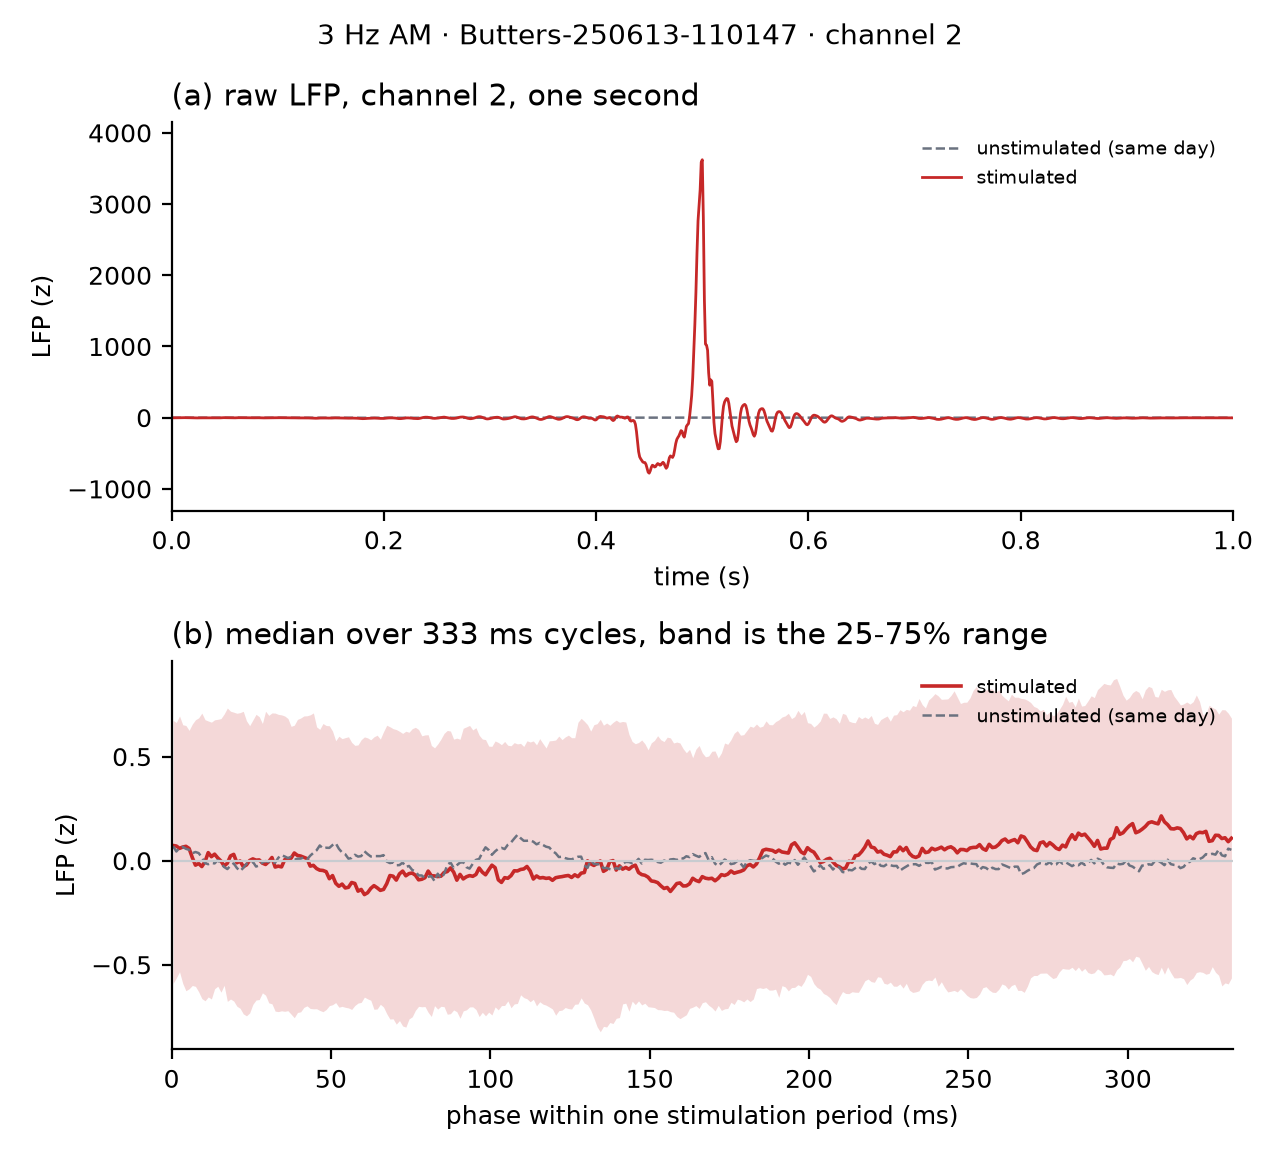
\includegraphics[width=\textwidth]{fig_artifact_3hz.png}
\caption{3~Hz stimulation day, worst channel. (a) one second of raw LFP around the largest transient, against the same-day unstimulated recording on the same channel. (b) the whole stimulation recording folded at the 333~ms period: the line is the median over cycles and the band the interquartile range, so a handful of multi-thousand-$z$ transients cannot set the curve. Red is the stimulated recording; the grey dashed line is the same-day unstimulated reference; the red band is the 25--75\% range (not clipped). The fold is flat, so the artifact carries no stable periodic template to estimate; what the decoder has to survive is the transient and its slow decay in (a).}\label{fig:artifact3}
\end{figure}

\begin{figure}[htbp]\centering
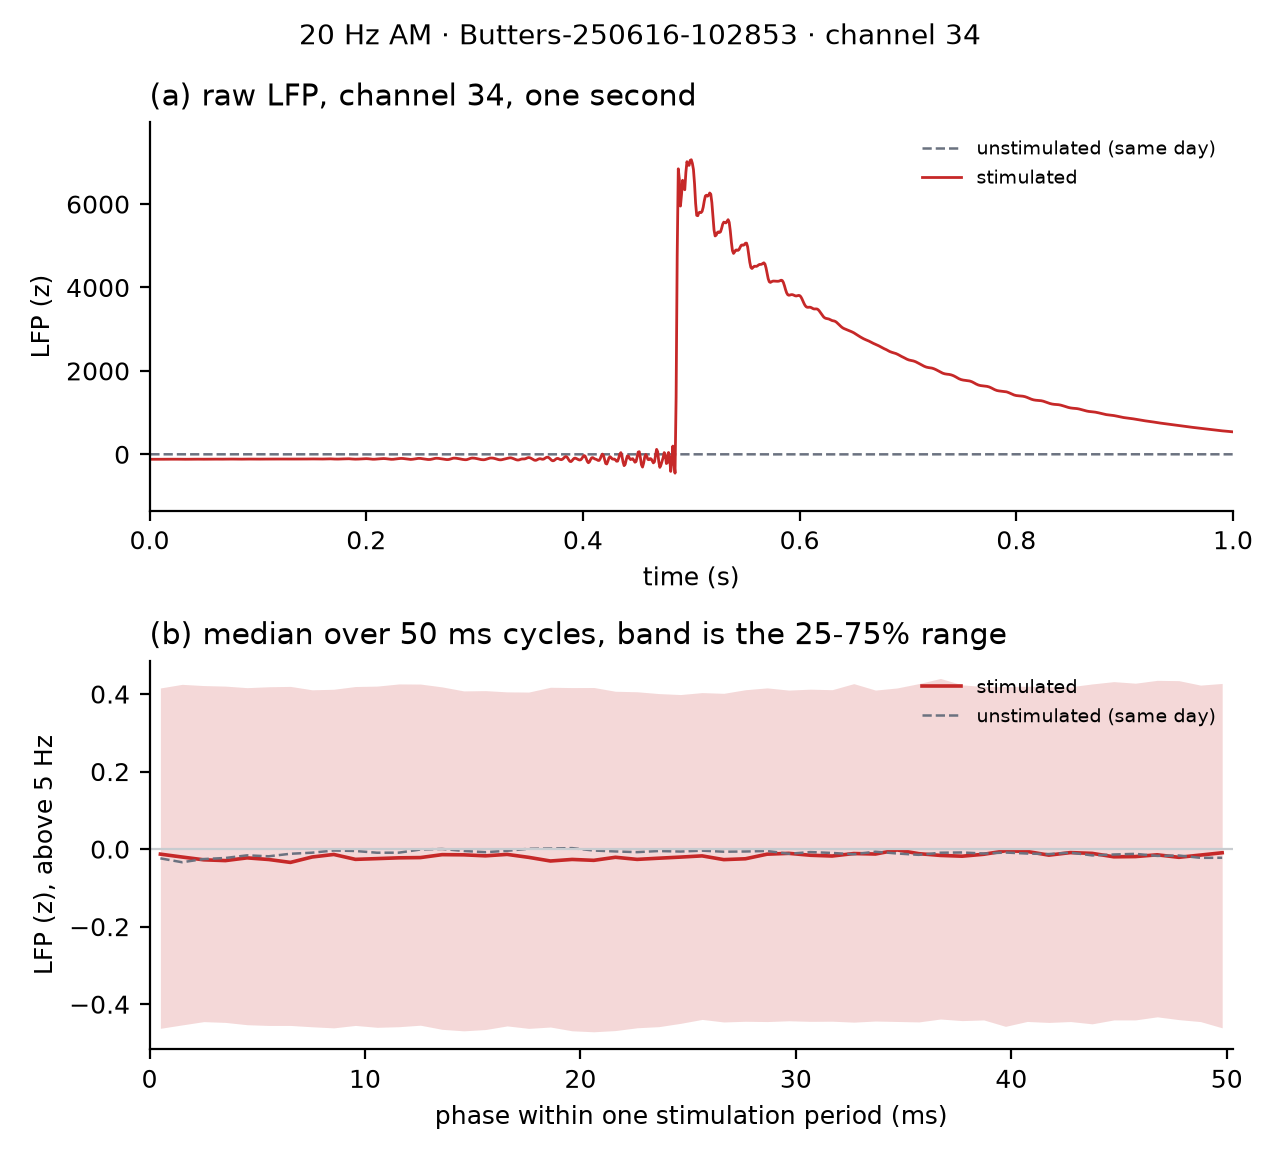
\includegraphics[width=\textwidth]{fig_artifact_20hz.png}
\caption{20~Hz stimulation day, worst channel. (a) one second of raw LFP around the largest transient: a step to about 7000~$z$ followed by a decay of several hundred milliseconds, so one transient outlasts many 50~ms periods. (b) the whole recording folded at the 50~ms period and high-passed above 5~Hz to remove the slow step; the line is the median over cycles and the band the interquartile range. Red is the stimulated recording; the grey dashed line is the same-day unstimulated reference; the red band is the 25--75\% range (not clipped).}\label{fig:artifact20}
\end{figure}

\begin{table}[htbp]\centering
\caption{Cycle-averaged artifact amplitude and peak transients in robust $z$-units.}
\small
\begin{tabular}{@{}lcccccc@{}}\toprule
Modulation & Period & Worst ch. & Avg. worst & Avg. median & Avg. clean & Peak transient \\ \midrule
3 Hz  & 333 ms & 2  & 3.1~z & 0.05~z & 0.04~z & 3622~z \\
20 Hz & 50 ms  & 34 & 2.0~z & 0.04~z & 0.02~z & 7064~z \\
\bottomrule\end{tabular}\label{tab:artifact}
\end{table}

PARRM~\cite{dastinvanrijn2021} exploits the repetition. Average the recording at the same
phase across many modulation cycles: neural and movement-related activity wanders from cycle
to cycle and averages out, while the artifact sits at the same phase every cycle and survives.
The average is a template of the artifact; subtract the template, per channel and per phase,
and what remains is nominally artifact-free. In the implementation used here the subtracted
component is a per-window gain times a mean template, with gains fitted in 1~s windows. Two
properties matter downstream. PARRM needs no labels, no kinematics and no calibration trials.
And it cannot distinguish artifact at phase $\theta$ from brain activity at phase $\theta$:
anything phase-locked to the stimulus is removed along with the artifact. On this dataset the
filter removes a median 17\% of the power in the modulation bin at 20~Hz and about 5\% at
3~Hz, while a sham filter applied to unstimulated data at the same period removes essentially
none, so the cleaning is real but partial.

\section{Decoding task, partitions and statistics}
\label{app:design}

The target is the velocity of the index fingertip, $(v_x,v_y)$, in screen cm/s, sampled in
50~ms bins from $0.5$~s before to $1.5$~s after the go cue, giving 40 bins per trial. Two
input representations are used, and the distinction organises the results. \emph{Spectral
features} are, per electrode and bin, the mean LFP over the preceding 256~ms and seven log
band powers between 1 and 200~Hz, computed causally: eight numbers per electrode per bin, 280
per bin, 2\,800 for a bin plus its nine predecessors. The \emph{raw waveform} is the 2\,000
LFP samples of the window per electrode, 35 channels, standardised per channel within the
session.

Sessions are partitioned by day into fixed train, validation and test sets; days are held
out, not trials. The test set contains 14 stimulation-on sessions, seven per modulation
frequency. Each is matched to the no-stimulation recording from the same day --- five
distinct recordings, since the three or four stimulated sessions of a day share one --- which
no decoder trains on. Scoring a decoder there gives the \emph{clean} column used throughout:
same decoder, same day, no artifact.

Within a stimulation session the first two blocks (20 trials) form a calibration pool and the
last three (30 trials) the query set, which is never used for fitting. For each session and
each $k\in\{2,5,10,20\}$ we sample subsets of $k$ trials from the pool: ten distinct subsets
for $k<20$, the whole pool for $k=20$, giving 434 partitions over the 14 sessions. Each is a
\emph{draw}, scored on that draw's 30 query trials. $k$ is a dose--response axis: the session
and the query trials stay fixed and only the labelled stimulated data changes.

Two levels of nesting must be respected. The ten draws within a session are correlated by
construction --- a $k=2$ draw is contained in the corresponding $k=5$ draw, and all ten at
$k=20$ are the same set --- and five seeds of a network are not independent evidence about
the data. Seeds and draws are therefore averaged \emph{inside} a session, and the 14 sessions
(seven per frequency) are the sample. Intervals are percentile intervals from 2\,000 bootstrap
resamples of sessions; resampling draws or seeds instead would shrink them by roughly
$\sqrt{10}$ and manufacture significance.

\begin{table}[htbp]\centering
\caption{Task 4 dataset, tensor shapes, splits, and calibration protocol ($C=35$ channels, $T=2{,}000$ samples, $N=40$ 50\,ms bins, $V=2$ velocity axes).}
\label{tab:datapipeline}
\footnotesize
\begin{tabular}{@{}p{0.22\textwidth}p{0.72\textwidth}@{}}
\toprule
Component & Specification \\
\midrule
\multicolumn{2}{@{}l}{\textbf{(a) Preprocessing and Tensor Shapes}} \\
Recordings \& Scaling & 70 sessions (1\,kHz raw LFP); 35 fixed motor-cortex channels centered and scaled per recording by median and MAD ($z$-units). \\
Inputs & Window $[t_{\mathrm{go}}-0.5,\, t_{\mathrm{go}}+1.5]$\,s ($40 \times 50$\,ms bins): raw LFP $(N_{\mathrm{trials}}, 35, 2000)$ for EEGNet; lagged spectral/LMP features $(N_{\mathrm{trials}}, 40, 2800)$ for window models ($8\text{ features} \times 35\text{ ch} \times 10\text{ lags}$). \\
Targets \& Mask & Binned fingertip velocity $(v_x, v_y)$ in cm/s, shape $(N_{\mathrm{trials}}, 40, 2)$, paired with binary validity mask $(N_{\mathrm{trials}}, 40)$. \\
\midrule
\multicolumn{2}{@{}l}{\textbf{(b) Date-Grouped Splits (70 Sessions Across 26 Days)}} \\
Train / Val (21 days) & \textbf{Train (18d):} 42 sessions (14 OFF, 13 at 3\,Hz, 15 at 20\,Hz). \textbf{Val (3d):} 9 sessions (3 OFF, 2 at 3\,Hz, 4 at 20\,Hz). \\
Test (5 days) & 19 sessions: 5 OFF, 7 at 3\,Hz, 7 at 20\,Hz (1, 3, 3, 3, 4 ON sessions/day, each paired with its day's OFF reference). \\
\midrule
\multicolumn{2}{@{}l}{\textbf{(c) Calibration Draws and Model Batching}} \\
Calibration Partitions & Across 14 test ON sessions: first 20 trials = calibration pool; final 30 trials = fixed query set. For $k \in \{2, 5, 10, 20\}$: 10 subsets for $k < 20$ and 1 full-pool draw for $k = 20$ ($434$ partitions). \\
Training \& Batching & \textbf{Causal EEGNet:} 560 train / 150 val OFF trials (batch 16; $F_1=8, D=2, F_2=16, K_1=500, K_2=62$, pool $2\times 25, p=0.25$). \textbf{Window models:} valid bins $(N_{\mathrm{valid}}, 2800)$; batch 256 (MLP/GRU) or closed-form (ridge). \\
\bottomrule
\end{tabular}
\end{table}


\begin{figure}[htbp]\centering
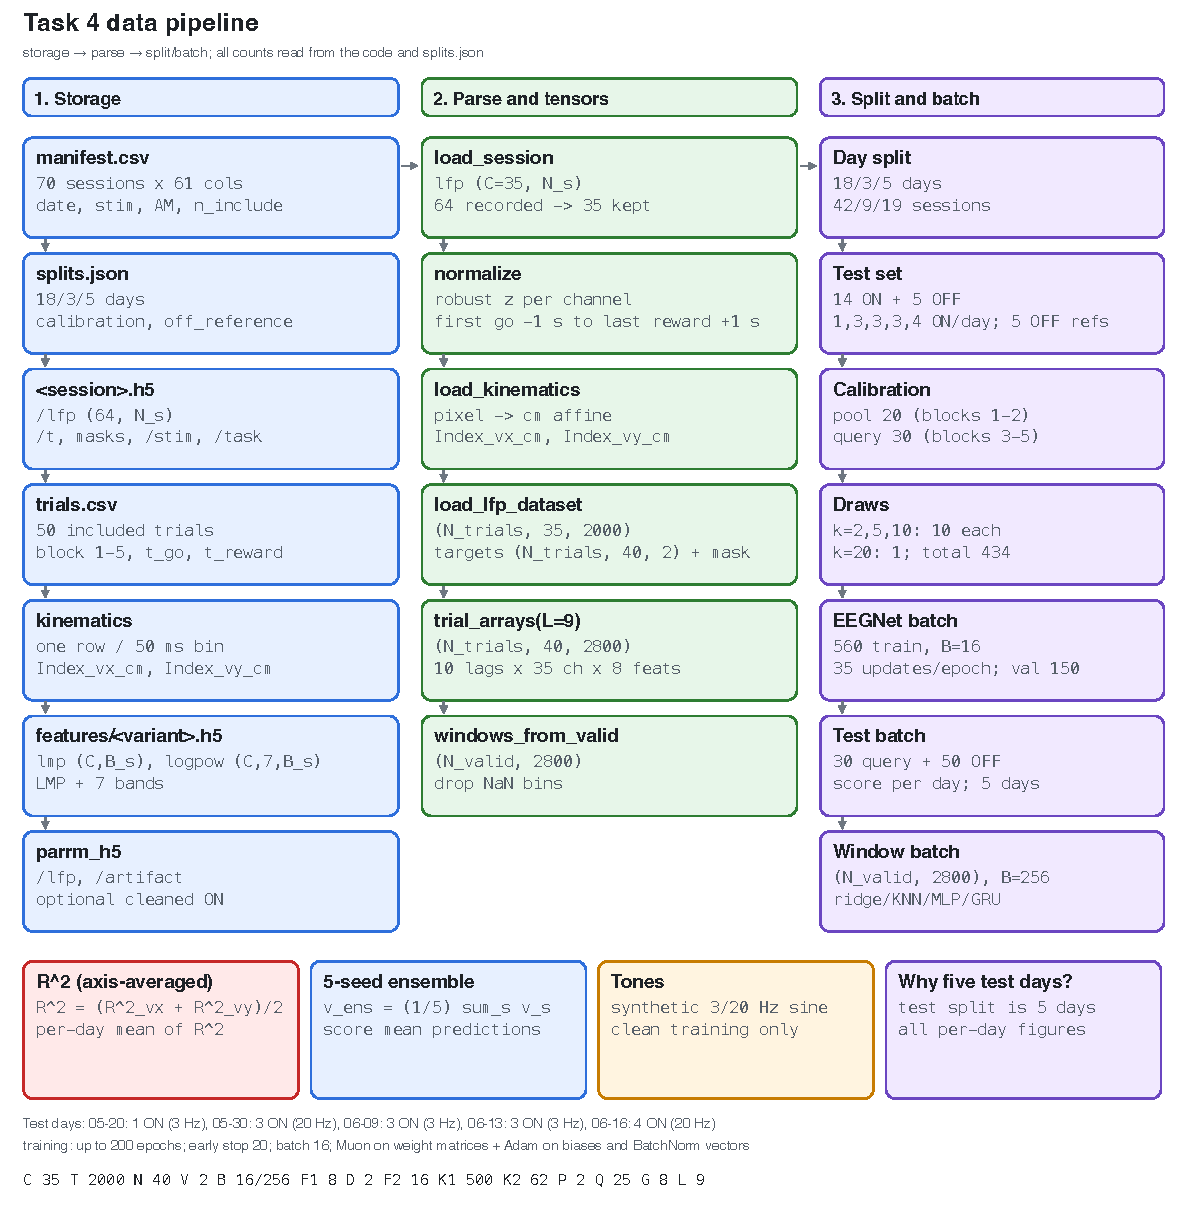
\includegraphics[width=\textwidth]{data_pipeline.pdf}
\caption{Task 4 data path. Column 1 is what is stored; column 2 is how each file becomes a tensor; column 3 is how the 26 days, 70 sessions, 14 test ON sessions, 5 shared OFF references, 20-trial pool, 30-trial query, and 434 draws are batched. The callouts define the axis-averaged $R^2$, the five-seed prediction ensemble, the synthetic tone augmentation, and why every per-day figure uses the same five test days.}\label{fig:datapipeline}
\end{figure}



\begin{table}[htbp]
\centering
\caption{Partition structure across the 14 test sessions (434 total partitions). All evaluations score the same 30 held-out query trials per session; $k=20$ uses the entire calibration pool, yielding one draw per session.}
\begin{tabular}{@{}cccc@{}}
\toprule
$k$ & Query trials scored & Draws per session & Total partitions \\ 
\midrule
2  & 30 & 10 & 140 \\ 
5  & 30 & 10 & 140 \\ 
10 & 30 & 10 & 140 \\ 
20 & 30 & 1  & 14  \\
\bottomrule
\end{tabular}
\label{tab:draws}
\end{table}

Absolute accuracy is low, and that constrains every claim. Fitting and testing on different
trials of the same \emph{unstimulated} session, with no stimulation and no cross-day transfer,
reaches only $\Rtwo\approx0.067$, ranging 0.039--0.126 across days. Speed is roughly ten times
more decodable than per-bin velocity, and the camera yields about 1.2 confident frames per
50~ms bin while instantaneous velocity has outliers beyond $\pm140$~cm/s, so a
central-difference velocity at that frame rate is noise-dominated. A difference of 0.01 is at
the resolution limit and 0.001 is not measurable; small differences are reported with paired
intervals and their direction is not interpreted.

\section{EEGNet architecture and training}\label{app:arch}\label{sec:eegnet}

\subsection{Causal EEGNet architecture}\label{sec:arch}

\begin{center}
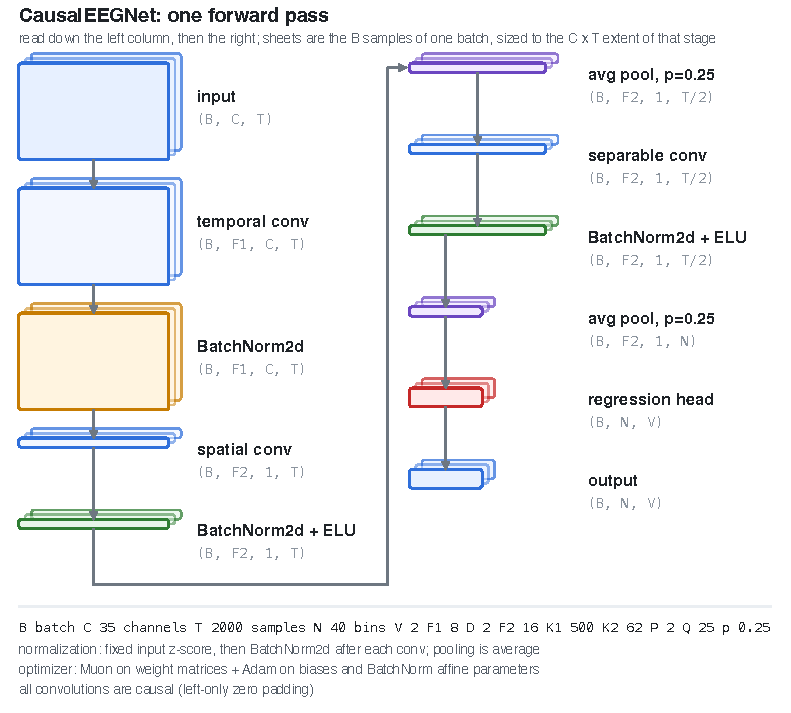
\includegraphics[width=0.68\textwidth]{eegnet_block_diagram.pdf}
\captionsetup{hypcap=false}
\captionof{figure}{Causal EEGNet forward pass (read down the left column, then the right). Stacked sheets denote batch $B$; each sheet is drawn at the real extent of its stage, so the height falls from $C=35$ channels to one and the width from $T=2{,}000$ samples to $N=40$ 50-ms bins and finally $(B,N,V)$. Pooling is average ($P=2$, then $Q=25$); dropout is $p=0.25$; all convolutions are causal.}\label{fig:arch}
\end{center}
We adapt \texttt{braindecode}'s EEGNet into a causal, per-bin regressor (5{,}922 parameters in the forward pass, stored as 6{,}005 scalars because the unit-norm spatial filter is parametrised by a direction and a length; Fig.~\ref{fig:arch}). The Causal EEGNet is an eleven-stage CNN with ELU activations.

The \emph{temporal convolution} slides a learned $1\times K_1$ filter ($K_1=500$, i.e.\ 500~ms) along time and reads all $C=35$ channels at once, producing $F_1=8$ feature maps; this is the stage that learns the shape of a temporal pattern. The \emph{spatial convolution} is depthwise with a $C\times1$ kernel, so each map becomes its own weighted mix of electrodes rather than a mix of maps; with depth multiplier $D=2$ this gives $F_2=F_1D=16$ maps and collapses the channel axis to one row. The \emph{separable convolution} pairs a $1\times K_2$ depthwise filter ($K_2=62$) along time with a $1\times1$ pointwise convolution, filtering each map's time course and then recombining across maps. The two \emph{pool\,+\,(dropout)} stages are \emph{average} pooling by $P=2$ and then by $Q=25$ with dropout $p=0.25$, which is what sets the output rate. The \emph{regression head} is a $1\times1$ convolution from $F_2=16$ maps to $V=2$ values, so the output is one $(v_x,v_y)$ pair per bin. Setting \texttt{final\_conv\_length=1} with two output channels and pooling factors of 2 and 25 maps $T=2{,}000$ input samples onto $N=40$ 50-ms velocity bins, one velocity pair per step. Fig.~\ref{fig:conv} draws the left padding and the kernel at the first, middle, and last output positions.

\begin{figure}[htbp]\centering
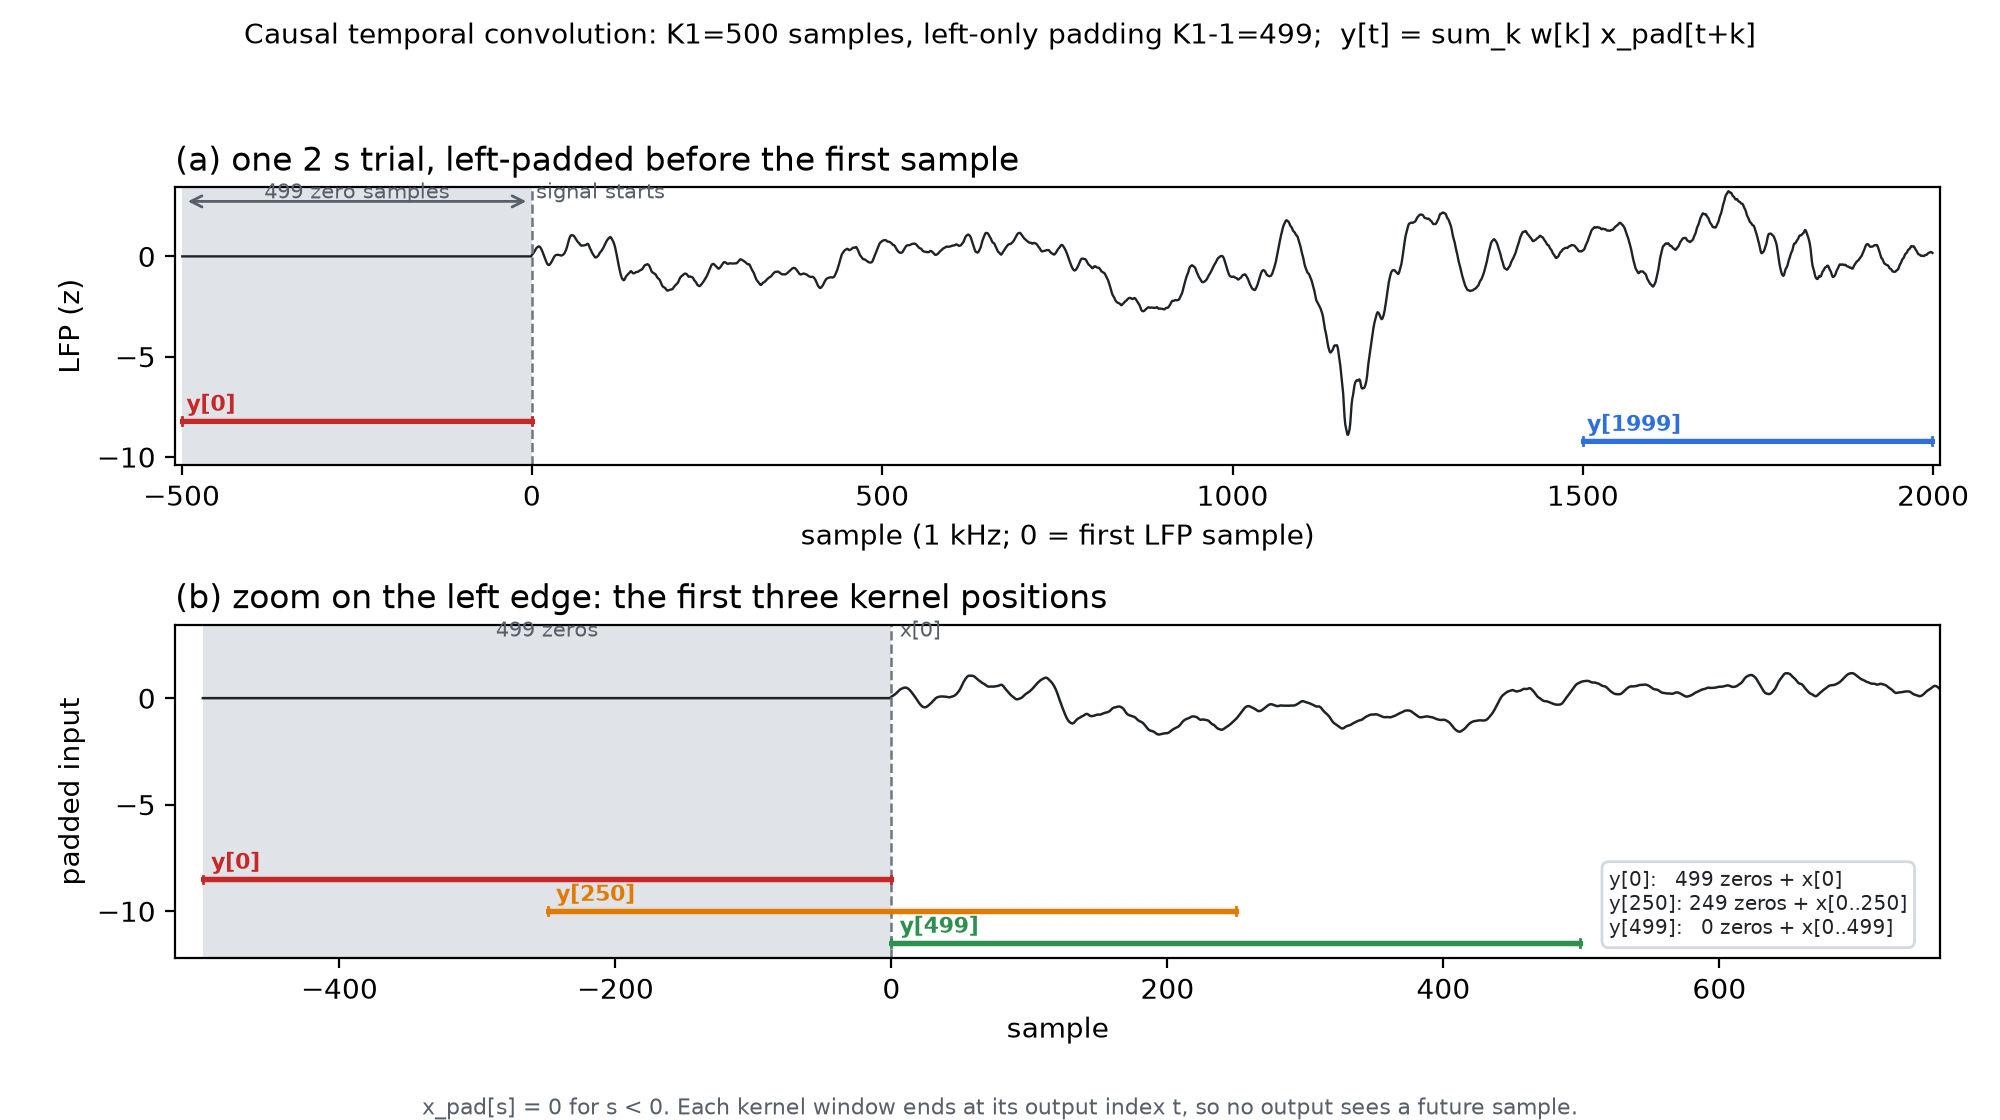
\includegraphics[width=\textwidth]{causal_convolution.png}
\caption{One causal temporal convolution on a single 1D LFP trial. The input is left-padded with $K_1-1=499$ zeros (grey); the $1\times K_1$ kernel ($K_1=500$ samples, 500~ms) slides left to right. The first output $y[0]$ sees 499 zeros plus $x[0]$; $y[250]$ sees 249 zeros plus $x[0..250]$; after 500 samples the kernel is fully inside the signal. No output sees a future sample. The same left-only scheme is used for the $K_2=62$ separable convolution.}\label{fig:conv}
\end{figure}

BatchNorm2d follows each convolution; it is a normalisation layer, not an optimizer. The two optimization algorithms are Muon, which updates the 2-D weight matrices via an orthogonalised update, and Adam, which updates the 1-D vectors (biases and the BatchNorm scale/shift parameters). Muon is not applied to 1-D vectors because the orthogonalisation is defined for matrices; Adam handles them at a small learning rate. The input z-score is a fixed per-channel preprocessing step, BatchNorm2d is a learned normalisation inside the network, and Muon/Adam are optimizers: they act at different stages and are not alternatives.

Replacing symmetric padding with left-only zero-padding before unpadded convolutions ensures each prediction depends strictly on current and past samples: $K_1-1$ zeros are added at the early edge for the $1\times K_1$ filter and $K_2-1$ for the $1\times K_2$ one. Spatial filters are projected onto the unit $\ell_2$-sphere after every gradient step, so only their direction is learned and never their scale; every saved model sits at exactly 1.000.


\subsection{Training objective and hyperparameter selection}\label{sec:loop}
Because camera tracking intermittently drops the fingertip, we mask missing targets ($m_b=1$ on valid bins, $M=\sum_b m_b$) in the mean squared error loss and evaluate axis-averaged $R^2$:
\begin{equation}
L = \frac{1}{M}\sum_b m_b\,\lVert\hat{\mathbf{v}}_b-\mathbf{v}_b\rVert^2, \qquad
R^2 = \tfrac{1}{2}\bigl(R^2_{v_x}+R^2_{v_y}\bigr), \quad
R^2_{\mathrm{axis}} = 1 - \frac{\sum_b (y_b-\hat{y}_b)^2}{\sum_b (y_b-\bar{y})^2}.
\label{eq:r2}
\end{equation}
Averaging $R^2$ across axes prevents the higher-variance component from dominating, where $R^2=0$ corresponds to predicting the bin mean $\bar{y}$. All reported $R^2$ values use this axis average. A per-day value is the mean of the session-level $R^2$ over the sessions of that day, not a single pooled $R^2$ over all trials; on the test split there are five such days, so every per-day figure shows the same five days.

We train the models for up to 200 epochs on 560 trials (batch size 16; 35 updates/epoch) using Muon for matrix parameters and Adam for vectors under a cosine learning rate schedule decaying to 1\% (the split/batch steps are summarised in Appendix Fig.~\ref{fig:datapipeline}). We checkpoint the best validation $R^2$ across 3 held-out sessions and early-stop after 20 epochs without a $10^{-4}$ improvement. An eight-configuration sweep over temporal kernel length, depth multiplier, and dropout (Table~\ref{tab:sweep}) selects a 500~ms kernel, depth multiplier 2, and dropout 0.25 ($R^2 = +0.1463$), though its $+0.0112$ margin over the default ($+0.1351$) lies within cross-seed variance (\S\ref{sec:seeds}).

For a trained model with per-bin prediction $\hat{\mathbf{v}}^{(s)}_b$ from seed $s$, the five-seed ensemble is
\begin{equation}
\hat{\mathbf{v}}^{\mathrm{ens}}_b = \frac{1}{5}\sum_{s=0}^{4}\hat{\mathbf{v}}^{(s)}_b,
\label{eq:ensemble}
\end{equation}
and the reported ensemble $R^2$ is computed on these averaged predictions. Tone augmentation (\texttt{+ tones}) adds a random-phase synthetic 3~Hz or 20~Hz sine to clean training trials, leaving target velocities unchanged, so the network meets interference at the frequencies stimulation injects without any stimulated label (Fig.~\ref{fig:toneaug}). Appendix~\ref{app:tones} gives the amplitude and channel-gain ranges.

\begin{table}[htbp]\centering
\caption{Architecture sweep ranked by clean validation $R^2$.}
\begin{tabular}{@{}lccccc@{}}\toprule
Kernel & Depth & Dropout & Val.\ $R^2$ & Best epoch & Last epoch \\ \midrule
500 ms  & 2 & 0.25 & $+0.1463$ & 48  & 68  \\ 
250 ms  & 2 & 0.50 & $+0.1378$ & 108 & 128 \\
500 ms  & 2 & 0.50 & $+0.1351$ & 56  & 76  \\ 
250 ms  & 2 & 0.25 & $+0.1293$ & 70  & 90  \\
500 ms  & 2 & 0.75 & $+0.1155$ & 38  & 58  \\ 
1000 ms & 2 & 0.50 & $+0.1149$ & 56  & 76  \\
500 ms  & 1 & 0.50 & $+0.0943$ & 48  & 68  \\ 
1000 ms & 2 & 0.25 & $+0.0908$ & 11  & 31  \\
\bottomrule\end{tabular}\label{tab:sweep}
\end{table}


\begin{table}[htbp]\centering
\caption{Mean test $R^2$ (axis-averaged over $v_x,v_y$; dimensionless) across the 5 held-out days and 5 seeds, with day-level bootstrap 95\% CIs. The ensemble averages the five predictions before scoring.}
\small
\begin{tabular}{@{}lcc@{}}\toprule
Decoder (trained without stimulated labels) & Clean test $R^2$ & Stimulated test $R^2$ \\ \midrule
EEGNet, single-seed mean (5 seeds) & $+0.021\ [-0.053,+0.087]$ & $-0.192\ [-0.383,-0.001]$ \\
EEGNet, 5-seed prediction ensemble & $+0.070\ [+0.013,+0.118]$ & $-0.134\ [-0.326,+0.059]$ \\
EEGNet + synthetic tones (App.~\ref{app:tones}) & $+0.033\ [+0.008,+0.058]$ & $+0.032\ [-0.005,+0.072]$ \\
\bottomrule\end{tabular}\label{tab:baseline}
\end{table}

\subsection{Seed variance and validation curves}\label{sec:seeds}
Across five random seeds (governing weight initialization, batch order, and dropout), validation $R^2$ reaches $0.136 \pm 0.011$ (individual runs: $0.146, 0.140, 0.122, 0.145, 0.125$; stopping between epochs 68 and 103; Fig.~\ref{fig:curves}). This $\pm 0.011$ standard deviation defines our experimental noise floor. Fig.~\ref{fig:seedspread} shows the same five kept scores beside the tone-augmented runs.

\begin{figure}[htbp]\centering
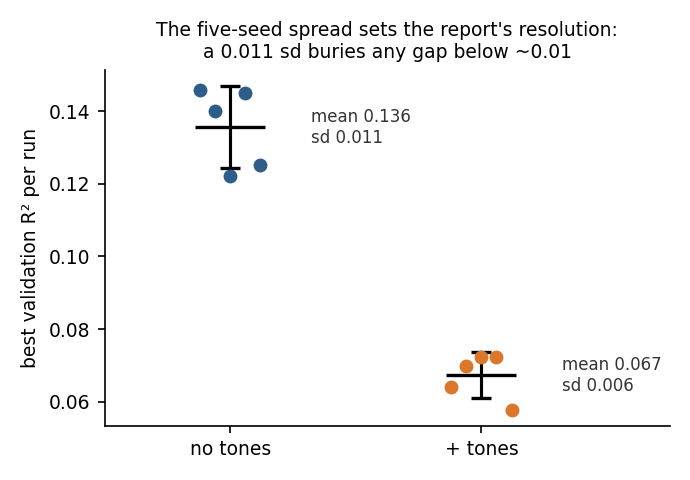
\includegraphics[width=0.72\textwidth]{fig_seed_spread.png}
\caption{Best validation $R^2$ for each of the five runs with and without tone augmentation. Each dot is one seed; the horizontal bar is the mean and the whisker $\pm1$ SD. The no-tone SD (0.011) is the resolution limit used in \S\ref{sec:seeds}; tone augmentation lowers the mean to $0.067\pm0.006$.}\label{fig:seedspread}
\end{figure}

\begin{figure}[htbp]\centering
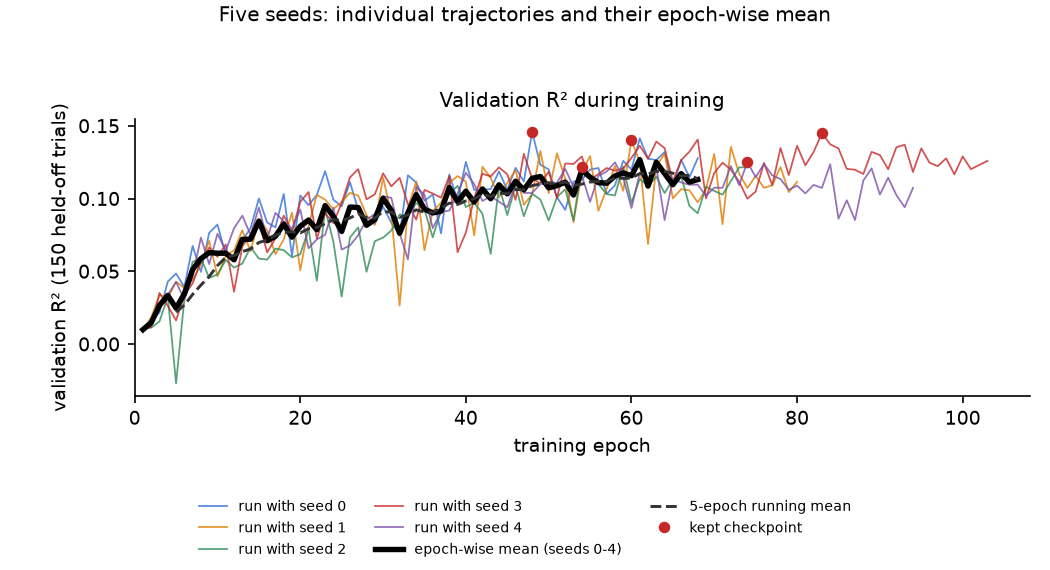
\includegraphics[width=\textwidth]{fig_val_curves.png}
\caption{Validation $R^2$ during training for the five seeds. One colour per run; the bold black line is the epoch-wise mean of the five runs, the dashed line its 5-epoch running average, and the red dots mark the checkpoint each run kept. The five kept scores average $0.136\pm0.011$ (reported in the text).}\label{fig:curves}
\end{figure}




\section{Other decoders}
\label{app:decoders}

\paragraph{Ridge.} A linear map from the 2\,800 standardised features of a 10-bin history to
the two velocities, fitted in closed form. The penalty is chosen once from 13 values spanning
$1$ to $10^6$ by mean validation $\Rtwo$ on stimulated validation sessions and then frozen, so
every draw is scored under the same penalty.

\paragraph{$k$-nearest neighbours.} Two variants, and the distinction is which labelled data
the model may look at. For an input bin the decoder returns the average velocity of the $k$
nearest \emph{stored} bins.

In the \emph{off-bank} variant the stored bins are the 17\,568 windows from the 14
stimulation-off training sessions --- the same data the ridge and neural decoders are fitted
on --- and no stimulated labels are used at all. The name refers to that bank of
stimulation-off examples: it is a non-parametric decoder whose entire model is a memory of
clean training windows. The neighbour count is chosen once on validation sessions ($k=200$),
and scoring a stimulated session means, for each query bin, averaging the velocity of its 200
nearest clean training bins.

In the \emph{in-context} variant the bank is instead the $k$ calibration trials of the draw
($k\le20$, roughly 680 bins at most). It has no parameters and no training, so it isolates how
much of any recovery is simply the presence of nearby labelled examples from the same session:
the off-bank and in-context rows differ only in which windows are in memory.

\begin{figure}[htbp]\centering
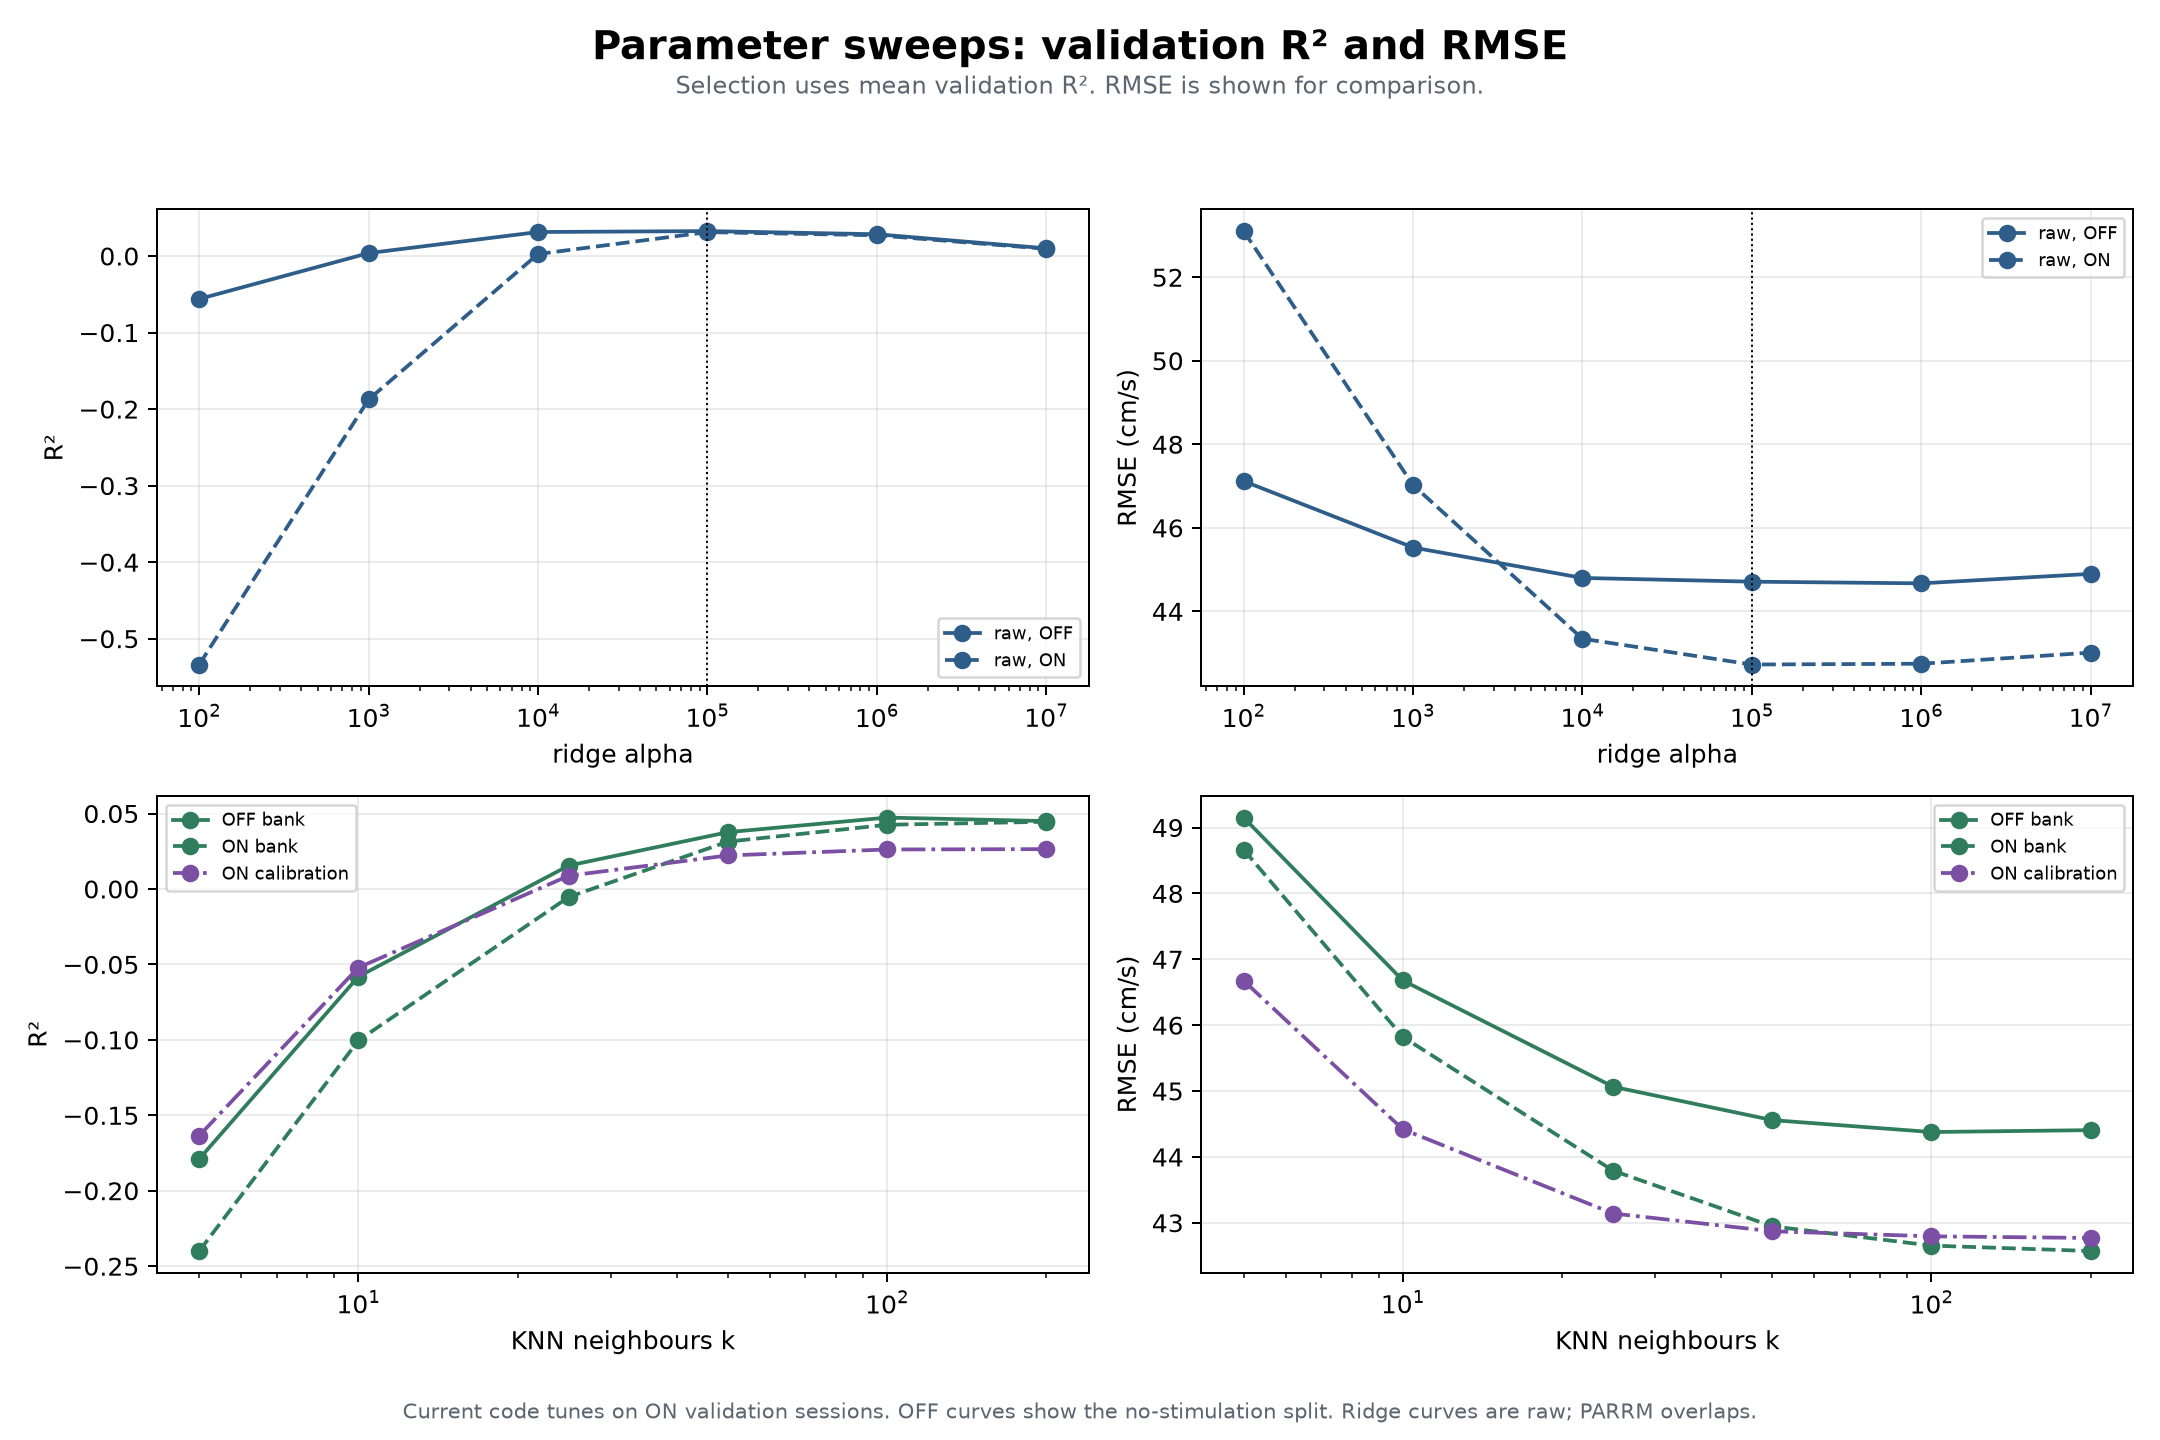
\includegraphics[width=\textwidth]{fig_parameter_sweeps.png}
\caption{Validation sweeps used to choose the ridge penalty and the KNN neighbour count. Top row: ridge $\alpha$ on a log scale for raw OFF (solid) and raw ON (dashed) input, with validation $R^2$ (left) and RMSE (right); the dotted line marks the selected $\alpha=10^5$. Bottom row: KNN neighbours for the OFF bank, ON bank, and ON calibration. Selection uses mean validation $R^2$; RMSE is shown for comparison. The current code tunes on ON validation sessions, and the OFF curves show the no-stimulation split for reference. PARRM overlaps the raw ridge curves.}\label{fig:sweeps}
\end{figure}

\paragraph{MLP.} Two dense layers (32 and 16 units, GELU, dropout) on the 2\,800 window
features, 90\,194 parameters, trained on stimulation-off training sessions with early stopping
on stimulation-off validation sessions.

\paragraph{GRU.} A single 128-unit GRU over the 40 bins of a trial, 157\,698 parameters,
reading the 280 per-bin spectral features. It sees the same information as the MLP but can
accumulate evidence across the trial.

\paragraph{Seed ensembles.} Every neural decoder is fitted five times from different random
initialisations; the five runs form the seeds. The ensemble \emph{averages the predictions},
not the scores: for each bin it takes the mean of the five networks' predicted $(v_x,v_y)$
pairs, and $\Rtwo$ is then computed on that averaged prediction against the targets. It is
not an average of five per-seed $\Rtwo$ values, and the two differ: averaging predictions
before scoring is strictly better here, because each seed's errors are partly independent and
cancel. On the recorded stimulation input the plain EEGNet moves from $-0.145$, the mean over
its five seeds, to $-0.082$ for the ensemble of those same five; on the clean input the same
comparison gives 0.037 against 0.082. The ensemble is better in both columns, and by more on
clean data than on stimulated data. This is not cosmetic: the seed spread of a single run is
comparable to the effects being measured, so the ensemble is the only quantity stable enough
to compare across decoders.

The sweep for the GRU (\S\ref{sec:gru}) is run at one seed and then the winner is
retrained across all five, so the sweep and the reported table describe the same network.

\section{Supervised recalibration: PARRM cleaning and ridge refitting}\label{app:parrm}\label{sec:parrm}
Standard recalibration removes the stimulation artifact without labels and then refits a linear decoder on $k$ labelled stimulation-on trials. PARRM removes the artifact by phase-averaging the recording across thousands of stimulation cycles—cancelling non-locked neural activity—and subtracting the resulting artifact template.

Because PARRM alone cannot rescue a clean-trained decoder (Task~3.2), we test whether it helps when refitting ridge regression from scratch on $k$ stimulated trials. For every partition in Appendix~\ref{app:design}, we train ridge on the $k$ calibration trials and evaluate on the 30 held-out query trials using either raw recorded features or PARRM-cleaned features (Table~\ref{tab:parrm}). Regularization is fixed on six separate stimulation-on validation sessions (Fig.~\ref{fig:sweeps}), and query $z$-scoring uses only each draw's $k$ calibration trials to prevent data leakage.



\begin{table}[htbp]\centering
\caption{Query-trial $R^2$ on stimulated recordings (mean across 14 sessions and 10 draws, with hierarchical bootstrap 95\% CIs).}
\begin{tabular}{@{}clcc@{}}\toprule
$k$ & Recorded ON & PARRM ON & Diff. \\ \midrule
2  & $+0.0038\ [+0.0007,+0.0072]$ & $+0.0037\ [+0.0005,+0.0071]$ & $-0.0002$ \\
5  & $+0.0160\ [+0.0103,+0.0223]$ & $+0.0159\ [+0.0100,+0.0223]$ & $-0.0002$ \\
10 & $+0.0290\ [+0.0205,+0.0386]$ & $+0.0286\ [+0.0200,+0.0382]$ & $-0.0004$ \\
20 & $+0.0444\ [+0.0320,+0.0582]$ & $+0.0438\ [+0.0315,+0.0576]$ & $-0.0006$ \\
\bottomrule\end{tabular}\label{tab:parrm}
\end{table}

Supervised refitting raised the query $R^2$ from $+0.0038$ at $k=2$ to $+0.0444$ at $k=20$, and the same-day unstimulated score from $+0.0014$ to $+0.0309$. PARRM did not improve on recorded features at any $k$, trailing by $0.0002\text{--}0.0006$ with overlapping confidence intervals. Three factors explain this null result: (i)~within-session artifact amplitude drift leaves large template residuals (channel~64 reaches $z \approx 5300$); (ii)~template subtraction strips genuine phase-locked neural and movement responses alongside the artifact; and (iii)~ridge refitting already down-weights artifact-dominated channels independently.

\paragraph{Benchmarking scope and stress testing.}
Whereas \S\ref{sec:eegnet} evaluates zero-shot transfer ($k=0$) across all 50 trials, \S\ref{sec:parrm} measures supervised adaptation on $k$ calibration trials evaluated over the 30 query trials; together, they establish the zero-shot and supervised baselines for downstream architectures (in-context transformer, fine-tuning, LoRA, and GRU). All models are evaluated on identical partitions and stress-tested on semi-synthetic 3~Hz and 20~Hz recordings where the 35 decoded LFP channels are scaled to $10\times$ artifact amplitude via $\text{LFP}_{10\times} = \text{LFP}_{\text{recorded}} + 9\,\text{PARRM}_{\text{artifact}}$.




\section{\texorpdfstring{The $10\times$ artifact stress test}{The 10x artifact stress test}}
\label{app:tenx}

Real stimulation amplitude was fixed for every session, so the dataset cannot say what happens
if the artifact were larger. We build such a condition and use it as a controlled probe. For
each stimulation-on session, only the 35 decoded channels and only the \texttt{/lfp} dataset
change:
\begin{equation}
\mathrm{LFP}_{10\times}(t)=\mathrm{LFP}_{\mathrm{recorded}}(t)+(\sigma-1)A(t),
\qquad \sigma=10,
\end{equation}
where $A(t)$ is the PARRM artifact estimate. Every other dataset and attribute --- sample
times, stimulation channels, trial tables, kinematics --- is copied verbatim, so the same
trials, labels and query split apply. Because $\mathrm{recorded}=\mathrm{clean}+A$ holds to
within 3\% relative RMS, the result is close to $\mathrm{clean}+10A$: the same session with ten
times the estimated artifact.

This condition is not stronger stimulation, since no current was changed. It is not the tone
augmentation used in Section~\ref{sec:eegnet}, which adds a pure sine to \emph{training}
trials; here nothing is trained and the added waveform is the measured artifact with its own
harmonics, drift and spatial pattern. Nor is it ten times noisier in broadband power, because
the artifact is narrowband and already present: the standard deviation of the $10\times$
recording is only 1.1--1.5 times the recorded one, and the median-absolute-deviation ratio is
1.92 at 3~Hz and 1.29 at 20~Hz.

PARRM's estimate scales with the amplitude of the periodic component it estimates, so
re-running it on the amplified signal gives an estimate ten times larger:
\begin{align*}
\mathrm{PARRM}\left(\mathrm{LFP}_{10\times}\right)
&= \mathrm{LFP}_{10\times}-\sigma A
 = \left(\mathrm{recorded}+(\sigma-1)A\right)-\sigma A \\
&= \mathrm{recorded}-A
 = \mathrm{PARRM}\left(\mathrm{LFP}_{\mathrm{recorded}}\right).
\end{align*}
The re-estimated cleaning therefore returns exactly the recording we already had; no new file
is needed, and the identity holds on all 20 validation and test sessions to a worst relative
RMS error of $3.7\times10^{-8}$. The informative alternative is the mistake: reusing the
original $1\times$ template leaves $\mathrm{LFP}_{10\times}-A=\mathrm{recorded}+8A$, still
eight copies of the artifact.

If the added term is to be discussed as noise, its statistics should be measured rather than
assumed. We take $n(t)=9A(t)$ on stimulation-on samples, remove each channel's mean, and
report what remains (Table~\ref{tab:noise}).

\begin{table}[h]
\centering
\small
\caption{The added $10\times$ term after removing each channel's mean. ``Binned'' means
averaged into the 50~ms bins the decoders see. Medians over seven test sessions.}
\label{tab:noise}
\begin{tabular}{@{}lrr@{}}
\toprule
Quantity & 3~Hz & 20~Hz \\
\midrule
DC RMS before centring                  & 3.0  & 2.0 \\
AC RMS after centring                  & 43.4 & 20.2 \\
Fraction of AC variance explained by modulation phase & 0.12 & 0.42 \\
Fraction of AC variance at harmonics $k f_0$, $k\le10$ & 0.07 & 0.06 \\
Share of AC variance in the worst five channels & 0.47 & 0.47 \\
\midrule
Fraction of AC variance retained by 50~ms binning & 0.56 & 0.21 \\
Lag-1 autocorrelation of the binned term & 0.35 & 0.98 \\
RMS of the binned term                 & 32.7 & 9.7 \\
Binned term SNR against the cleaned LFP (dB) & $-0.1$ & $-10.2$ \\
MAD ratio, amplified over recorded     & 1.92 & 1.29 \\
\bottomrule
\end{tabular}
\end{table}

The term is not white: after centring, only 12\% (3~Hz) to 42\% (20~Hz) of its variance is
explained by the modulation phase, and only 6--7\% sits in the first ten harmonics, so it
behaves like a drifting gain times a template rather than a tone. It is not isotropic: about
half the variance sits in five of 35 channels. And most of it can disappear before the decoder
sees it, which is the subject of Appendix~\ref{app:mechanism}.

Scoring the same weights on four inputs, with nothing retrained, separates cleaning from the
ability to learn around the artifact (Table~\ref{tab:tenx}). Cleaning rescues the fixed
decoder and the ensemble ends above its own clean control, 0.106 against 0.082. Re-estimating
matters more than cleaning: reusing the original template leaves eight copies and stays
catastrophic. And the two fixes overlap, since the tone-augmented arm is already flat across
artifact amplitudes and gains nothing from cleaning. Ten times the artifact drives a fixed
raw-waveform decoder to $-3.2$, which is why the condition is useful as a stress test even
though it is artificial: it separates decoders that were already robust from those that were
merely lucky at the recorded amplitude.

\begin{table}[!t]
\centering
\small
\caption{Query-trial $\Rtwo$ with identical weights on four inputs. ``PARRM re-estimated''
cleans the amplified signal with a template fitted to it; ``$1\times$ reused'' cleans it with
the original template, leaving eight copies.}
\label{tab:tenx}
\begin{tabular}{@{}lrrrrr@{}}
\toprule
Decoder & recorded & $10\times$ & PARRM re-est. & $1\times$ reused & clean \\
\midrule
EEGNet, single seed      & $-0.145$ & $-3.244$ & $+0.050$ & $-2.944$ & 0.037 \\
EEGNet, 5-seed ensemble  & $-0.082$ & $-2.544$ & $+0.106$ & $-2.327$ & 0.082 \\
Tone-augmented, single   & $+0.030$ & $-0.322$ & $+0.026$ & $-0.246$ & 0.032 \\
Tone-augmented, ensemble & $+0.052$ & $-0.205$ & $+0.050$ & $-0.151$ & 0.048 \\
\bottomrule
\end{tabular}
\end{table}

\section{Complete results}
\label{app:results}

Table~\ref{tab:main} collects every decoder on the 30 query trials of each of the 14 test
sessions. Table~\ref{tab:dose} traces the two adaptive decoders across $k$; both are monotone
at every step and both are near zero at $k=2$, where two trials supply about 68 bins for
2\,800 inputs. The shape --- nothing until $k\approx10$, most of the gain between $k=10$ and
$k=20$ --- is what an underdetermined linear fit should look like, not a smooth learning
curve. That a parameter-free nearest-neighbour rule with the same 20 trials lands within 0.004
of ridge says the recovery does not depend on a well-specified model.

\begin{table}[!t]
\centering
\small
\caption{Query-trial $\Rtwo$ on stimulated recordings and on the matched clean recording.
``Adapts'' gives the number of labelled stimulated trials used; a dash means none.}
\label{tab:main}
\begin{tabular}{@{}llrrrr@{}}
\toprule
Decoder & Adapts & All (14) & 3~Hz (7) & 20~Hz (7) & clean \\
\midrule
Ridge, raw, no adaptation       & --- & $+0.008$ & $+0.025$ & $-0.010$ & 0.034 \\
Ridge, PARRM, no adaptation     & --- & $+0.002$ & $+0.025$ & $-0.020$ & 0.034 \\
$k$-NN, off bank                & --- & $+0.026$ & $+0.026$ & $+0.027$ & 0.028 \\
MLP, 5 seeds                    & --- & $+0.004$ & $+0.039$ & $-0.032$ & 0.045 \\
GRU, 5 seeds                    & --- & $+0.029$ & $+0.028$ & $+0.029$ & 0.033 \\
EEGNet, single seed             & --- & $-0.145$ & $-0.337$ & $+0.047$ & 0.037 \\
EEGNet, 5-seed ensemble         & --- & $-0.082$ & $-0.280$ & $+0.117$ & 0.082 \\
EEGNet, tone-augmented          & --- & $+0.030$ & $+0.031$ & $+0.030$ & 0.032 \\
\midrule
$k$-NN, in-context, $k=20$      & 20 & $+0.040$ & $+0.029$ & $+0.051$ & 0.027 \\
Ridge, raw, refit, $k=20$       & 20 & $+0.042$ & $+0.030$ & $+0.055$ & 0.031 \\
Ridge, PARRM, refit, $k=20$     & 20 & $+0.041$ & $+0.029$ & $+0.053$ & 0.030 \\
\bottomrule
\end{tabular}
\end{table}

\begin{table}[!t]
\centering
\small
\caption{Query-trial $\Rtwo$ against the number of labelled stimulated trials, mean over 14
sessions and 10 draws per session.}
\label{tab:dose}
\begin{tabular}{@{}llrrrr@{}}
\toprule
Decoder & Frequency & $k=2$ & $k=5$ & $k=10$ & $k=20$ \\
\midrule
Ridge, raw & 3~Hz  & $0.001$ & $0.010$ & $0.019$ & $0.030$ \\
Ridge, raw & 20~Hz & $0.002$ & $0.021$ & $0.038$ & $0.055$ \\
$k$-NN     & 3~Hz  & $-0.002$ & $0.005$ & $0.017$ & $0.029$ \\
$k$-NN     & 20~Hz & $-0.001$ & $0.010$ & $0.030$ & $0.051$ \\
\bottomrule
\end{tabular}
\end{table}

Two features of Table~\ref{tab:main} organise the rest. The unadapted spectral decoders split
by frequency: ridge is mildly positive at 3~Hz and negative at 20~Hz, i.e.\ worse than
predicting the mean, and taking the clean column as the ceiling the artifact costs ridge 0.039
at 20~Hz against 0.014 at 3~Hz. The raw-waveform decoder does the opposite, catastrophic at
3~Hz and fine at 20~Hz. The MLP mirrors EEGNet's asymmetry and the GRU has none: three
architectures, three signatures, with seed spread too small to explain them.

Cleaning adds nothing once labels are being spent. Refitting ridge on raw features gives
$+0.042$ and on cleaned features $+0.041$, a paired difference of $0.001$ that the spread
cannot resolve; across the whole $k$ range the difference never exceeds 0.001 and its sign
flips between frequencies. This is a narrow statement, not ``cleaning is useless''. A decoder
refitted on labelled stimulated trials can learn small weights on artifact-dominated channels
by itself, so cleaning overlaps with what the labels were going to buy. Cleaning matters most
exactly where labels are absent, and for a waveform-domain decoder it is then worth 0.19
$\Rtwo$ (Appendix~\ref{app:tenx}) rather than 0.001 --- the same intervention, a different
question.

Table~\ref{tab:paired} gives paired differences on aligned sessions. The GRU's advantage over
EEGNet is entirely a 3~Hz effect, with all seven sessions in the same direction and no
separation at 20~Hz. In the opposite direction the EEGNet ensemble beats the GRU at 20~Hz by
0.087 in six of seven sessions, so the stable deep baseline is not the best one; it is the one
whose failure is frequency independent. Twenty labelled trials beat the GRU overall but not
decisively, and not at 3~Hz.

\begin{table}[h]
\centering
\small
\caption{Paired differences in query-trial $\Rtwo$ with 95\% session-bootstrap intervals.
Positive means the first decoder is better.}
\label{tab:paired}
\begin{tabular}{@{}lrrr@{}}
\toprule
Comparison & All (14) & 3~Hz (7) & 20~Hz (7) \\
\midrule
GRU $-$ EEGNet              & $+0.174\,[0.063, 0.287]$ & $+0.365\,[0.282, 0.439]$ & $-0.017\,[-0.082, 0.041]$ \\
GRU $-$ EEGNet ensemble     & $+0.110\,[0.003, 0.223]$ & $+0.308\,[0.236, 0.378]$ & $-0.087\,[-0.132, -0.045]$ \\
Tones $-$ EEGNet            & $+0.175\,[0.074, 0.283]$ & $+0.367\,[0.300, 0.433]$ & $-0.017\,[-0.042, 0.011]$ \\
Ridge refit $-$ GRU         & $+0.014\,[-0.001, 0.028]$ & $+0.002\,[-0.013, 0.015]$ & $+0.026\,[0.002, 0.047]$ \\
$k$-NN $-$ ridge refit      & $-0.002\,[-0.011, 0.006]$ & $-0.000$ & $-0.004$ \\
\bottomrule
\end{tabular}
\end{table}

\subsection{Per-day zero-shot results}

The tables above score the fixed 30-trial query set, so that unadapted and adapted decoders share the same trials. Section~\ref{sec:eegnet} and the per-day figures below instead score all 50 stimulated trials per session and average over the five test days; the two protocols therefore differ in absolute $R^2$.

\paragraph{Test performance without stimulated training data.}
We first evaluate EEGNet models trained solely on unstimulated (clean) recordings, without any stimulation-on calibration trials (Table~\ref{tab:baseline}, Fig.~\ref{fig:perday}). Averaged across the 5 random seeds and 5 held-out test days, single-seed EEGNet achieves $+0.021$ $R^2$ on clean test days but drops to $-0.192$ under stimulation—19\% worse than predicting the session's mean velocity. Averaging the predicted velocity vectors across all 5 seeds at each 50-ms bin (\texttt{seed = -1}; Fig.~\ref{fig:ensemble}) reduces seed-to-seed prediction noise, raising the 5-day mean clean $R^2$ to $+0.070$ (gaining $+0.077$ on day 250520, where single-seed SD is 0.097) and stimulated $R^2$ to $-0.134$. Adding synthetic sine-wave interference during clean training (Appendix~\ref{app:tones}) prevents collapse under stimulation ($+0.032$ $R^2$), though clean $R^2$ drops to $+0.033$.

\begin{figure}[htbp]\centering
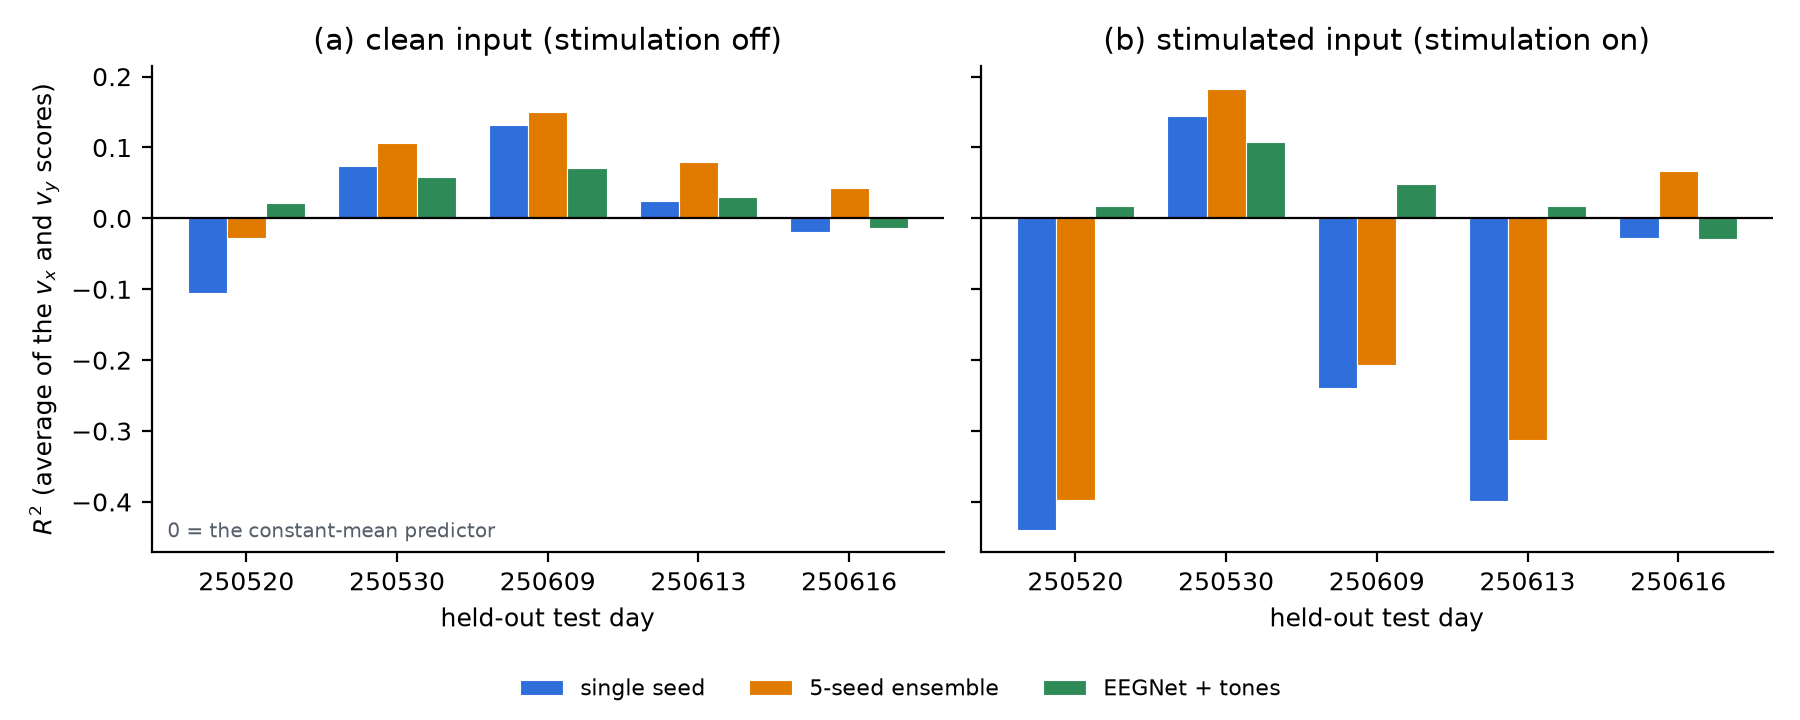
\includegraphics[width=\textwidth]{fig_perday_r2.png}
\caption{Per-day test $R^2$ on the five held-out test days. (a) clean input, the same-day stimulation-off recording. (b) stimulated input, the stimulation-on recording. Each bar is the mean of the session-level $R^2$ over the sessions of that day: blue is the mean of the five seeds, orange is the five-seed prediction ensemble of \eqref{eq:ensemble}, green is a decoder trained with synthetic tones (Appendix~\ref{app:tones}). Every $R^2$ is the average of the $v_x$ and $v_y$ scores, and $0$ is the constant-mean predictor.}\label{fig:perday}
\end{figure}

\begin{figure}[htbp]\centering
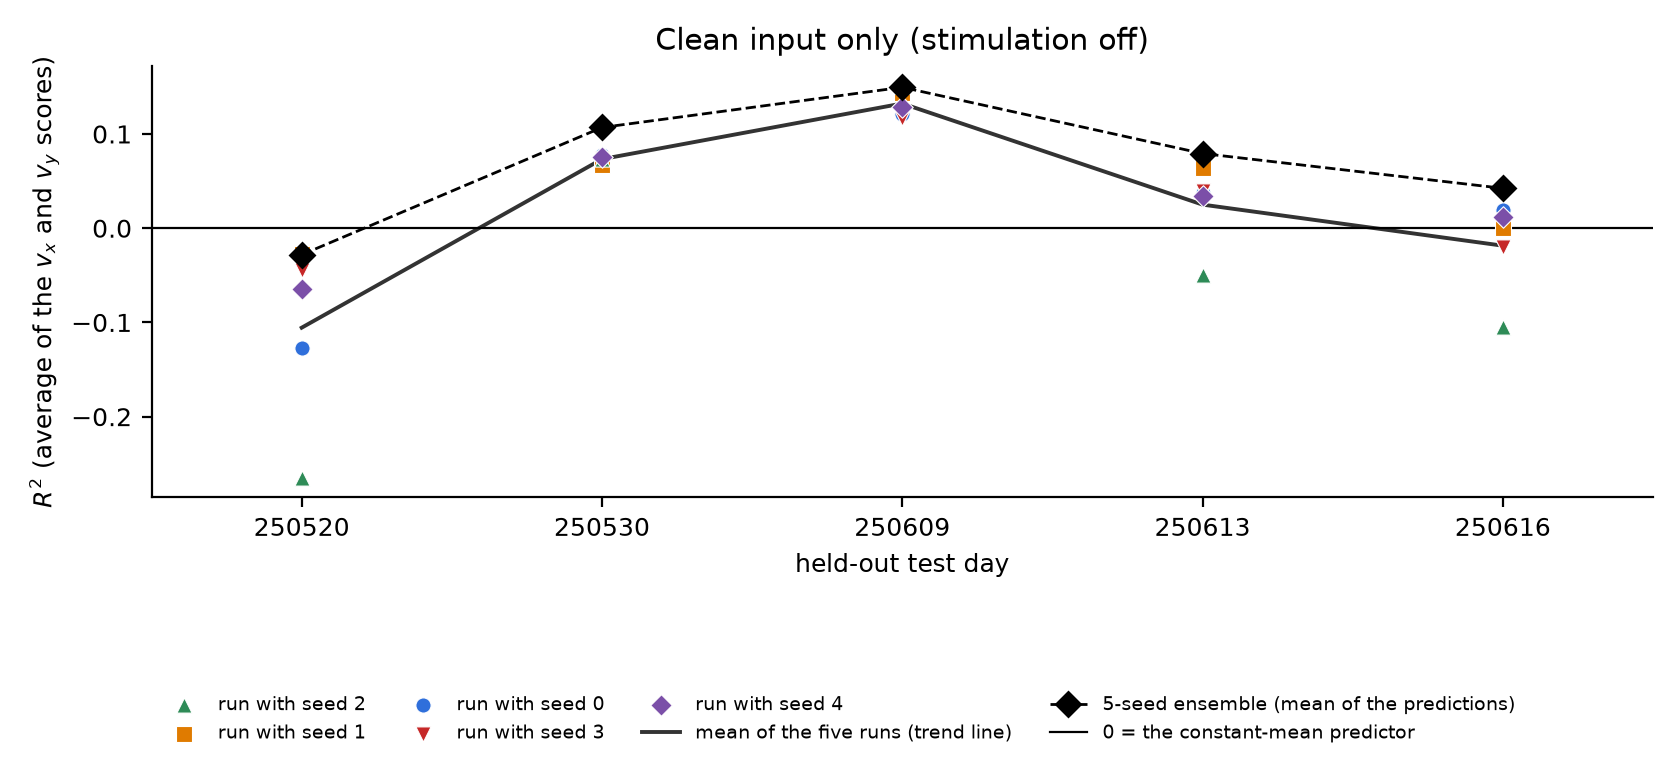
\includegraphics[width=\textwidth]{fig_ensemble.png}
\caption{Clean-input $R^2$ per held-out test day. All seeds are plotted at the same day position; colours and marker shapes distinguish them. The solid line joins the mean of the five seeds, and the black diamonds are the five-seed ensemble of \eqref{eq:ensemble}. The gap between the solid line and the diamonds is the gain from averaging predictions rather than scores. $R^2$ is the average of the $v_x$ and $v_y$ scores; $0$ is the constant-mean predictor.}\label{fig:ensemble}
\end{figure}

\paragraph{Velocity error in cm/s and comparison to ridge.}
In physical units, predicting the constant mean velocity yields a Euclidean speed RMSE ($\sqrt{e_{v_x}^2 + e_{v_y}^2}$) of $61\text{--}68\;\text{cm/s}$ across the 5 test days (Fig.~\ref{fig:r2rmse}, Table~\ref{tab:perday}). On clean recordings, the 5-seed EEGNet ensemble lowers 5-day mean RMSE by 3\% (up to 7\% on day 250609: 63.2 vs.\ 68.0~cm/s, $R^2 = +0.150$). Compared against the Task~3.1 ridge baseline—which uses causal local motor potentials and seven 1--200~Hz band powers across 10 lags—single-seed EEGNet trails by $-0.024$ $R^2$ on average across the 5 days (95\% CI $[-0.119, +0.047]$), beating ridge on 2 of 5 days and leading by $+0.017$ if the single-session day 250520 ($-0.106$ vs.\ $+0.084$) is excluded.

\begin{figure}[htbp]\centering
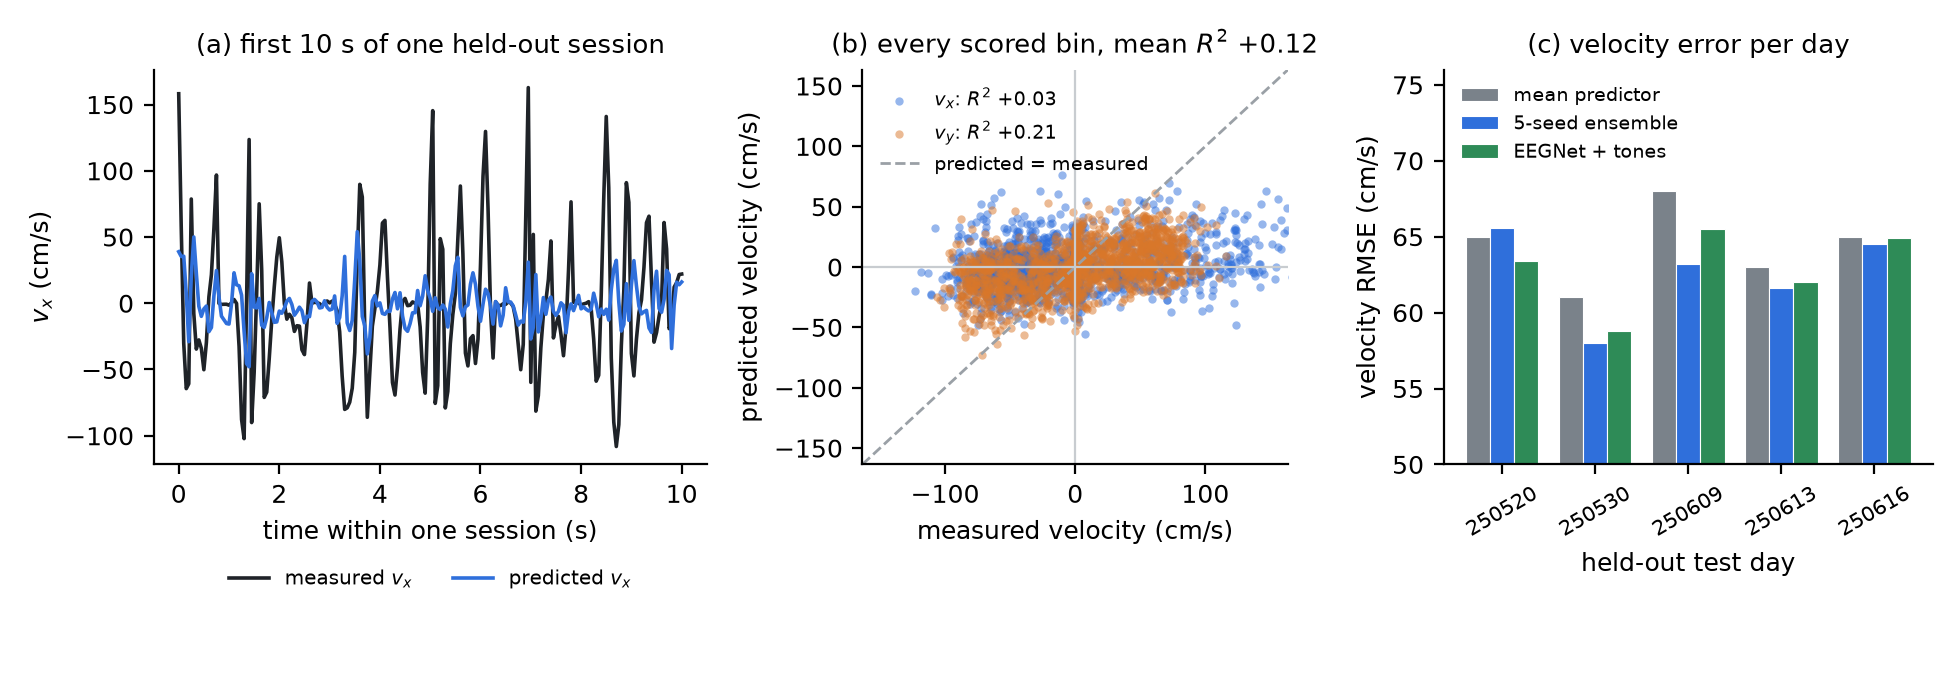
\includegraphics[width=\textwidth]{fig_r2_vs_rmse.png}
\caption{From $R^2$ to centimetres per second, all on clean input. (a) measured and predicted $v_x$ over the first 10~s of one held-out session. (b) predicted against measured velocity for every scored bin of that session, with the diagonal as a perfect forecast; the prediction is compressed toward zero, which is why $R^2$ stays positive while the scatter is wide. (c) per-day Euclidean velocity RMSE, $\sqrt{e_{v_x}^2+e_{v_y}^2}$, against the constant-mean predictor, whose error is $\sqrt{2}\,\mathrm{SD}(\text{speed})$. Day identity is on the axis because RMSE is not comparable across days of different speed.}\label{fig:r2rmse}
\end{figure}

\begin{table}[htbp]\centering
\caption{Per-day test performance across models (clean and stimulated $R^2$, plus clean RMSE in cm/s).}
\scriptsize
\setlength{\tabcolsep}{3pt}
\begin{tabular}{@{}lcccccccc@{}}\toprule
 & \multicolumn{5}{c}{Clean $R^2$} & \multicolumn{2}{c}{Clean RMSE (cm/s)} & Stim.\ $R^2$ \\
\cmidrule(lr){2-6}\cmidrule(lr){7-8}\cmidrule(lr){9-9}
Day & Ridge & Base.\ (SD) & Ens. & +Tones & Mean pred. & Ens. & +Tones & Base.\ / +Tones \\ \midrule
250520 & $+0.084$ & $-0.106\ (0.097)$ & $-0.028$ & $+0.022$ & 65.0 & 65.6 & 63.4 & $-0.439\ /\ +0.018$ \\
250530 & $+0.037$ & $+0.073\ (0.004)$ & $+0.107$ & $+0.058$ & 61.0 & 58.0 & 58.8 & $+0.145\ /\ +0.108$ \\
250609 & $+0.046$ & $+0.132\ (0.014)$ & $+0.150$ & $+0.071$ & 68.0 & 63.2 & 65.5 & $-0.240\ /\ +0.048$ \\
250613 & $+0.038$ & $+0.025\ (0.043)$ & $+0.079$ & $+0.030$ & 63.0 & 61.6 & 62.0 & $-0.399\ /\ +0.017$ \\
250616 & $+0.022$ & $-0.019\ (0.050)$ & $+0.042$ & $-0.014$ & 65.0 & 64.5 & 64.9 & $-0.027\ /\ -0.030$ \\
\bottomrule\end{tabular}\label{tab:perday}
\end{table}





\section{Synthetic tone augmentation}\label{app:tones}

To test whether training against periodic interference improves zero-shot transfer without using stimulated labels, we augment clean training trials with a synthetic sine wave at the measured stimulator frequencies (2.99~Hz and 19.90~Hz; periods of 333~ms [6.7 bins] and 50~ms [1.0 bin]), leaving target velocities unchanged. Each training trial receives a single random-phase tone with amplitude 0.5--3.0~z and channel-wise gain 0.5--1.5 (dimensionless). This matches the cycle-averaged artifact magnitude in Appendix~\ref{app:artifact} (2.0--3.1~z) while avoiding the 3{,}000--7{,}000~z peak transients that would otherwise saturate the network.

\begin{figure}[htbp]\centering
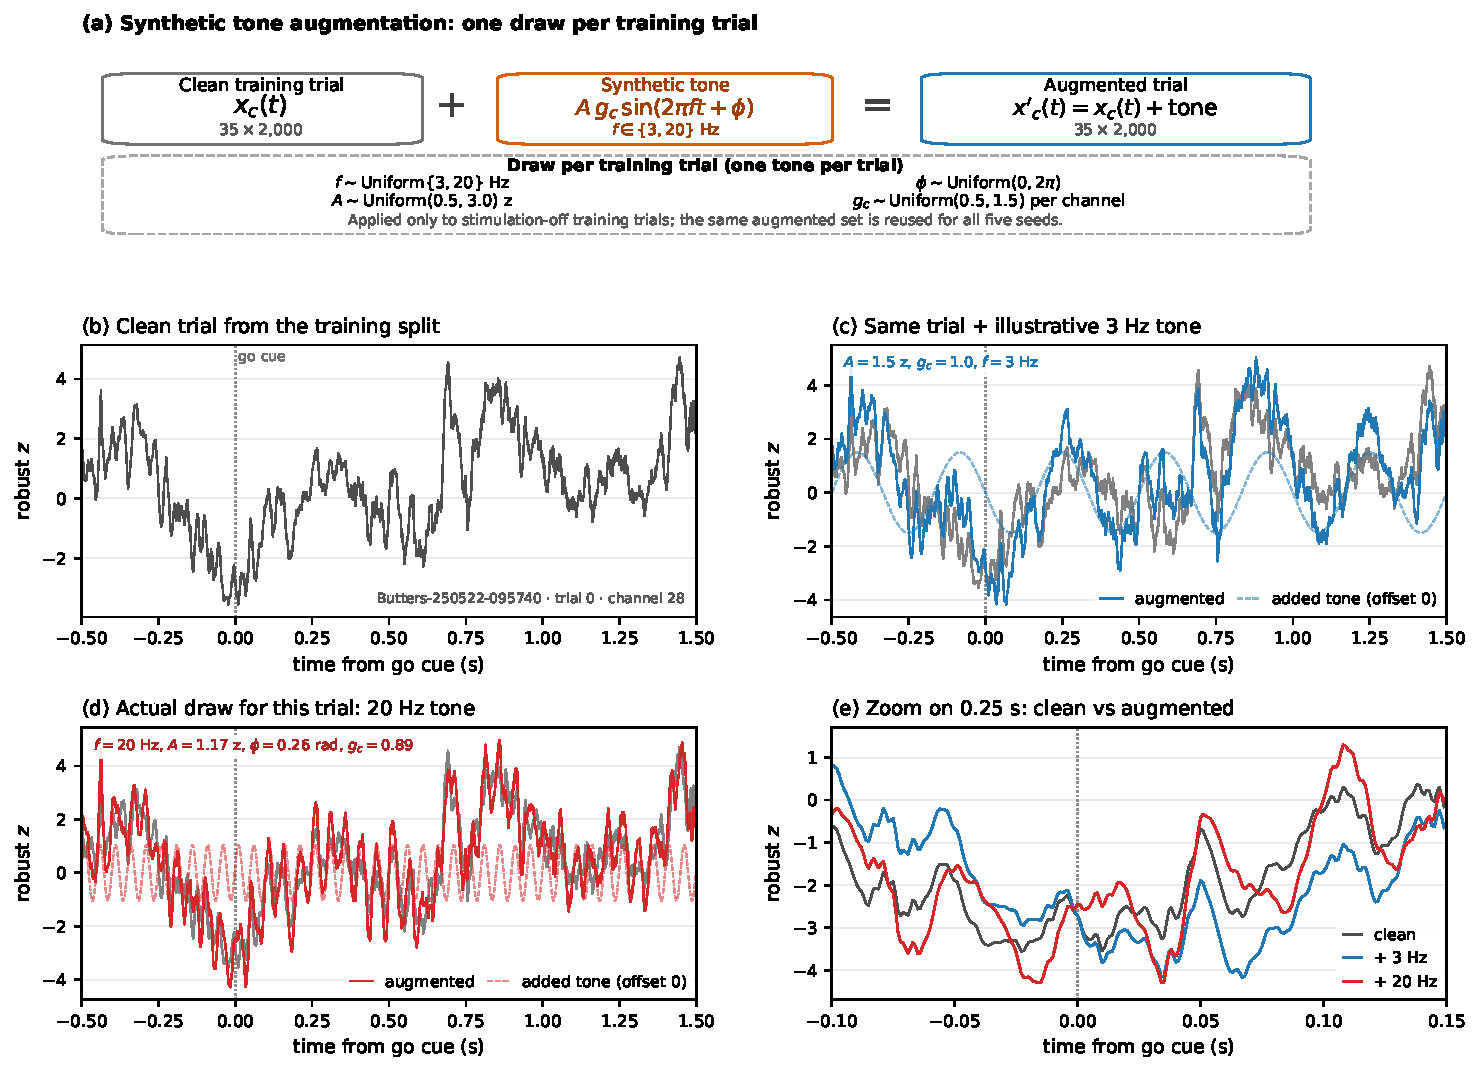
\includegraphics[width=\textwidth]{tone_augmentation.pdf}
\caption{Tone augmentation on a real stimulation-off training trial. (a) A clean trial $x_c(t)$ receives a synthetic tone $A g_c\sin(2\pi f t+\phi)$ to form $x'_c(t)$; the target velocities are unchanged. Each training trial draws one frequency $f\in\{3,20\}$~Hz, amplitude $A\in[0.5,3.0]$ robust $z$, phase $\phi\in[0,2\pi)$, and one gain $g_c\in[0.5,1.5]$ per channel. (b) The clean trial (session Butters-250522-095740, trial 0, channel 28). (c) The same trial with an illustrative 3~Hz tone ($A=1.5$~z, $g_c=1.0$). (d) The actual seed-0 draw for this trial: 20~Hz, $A=1.17$~z, $\phi=0.26$~rad, $g_c=0.89$. (e) A 0.25~s zoom comparing the clean and augmented traces. The dashed curves in (c)--(d) are the added tones, plotted at zero offset. The augmentation is applied only to the stimulation-off training set, and the same augmented set is reused across all five seeds.}\label{fig:toneaug}
\end{figure}

\begin{figure}[htbp]\centering
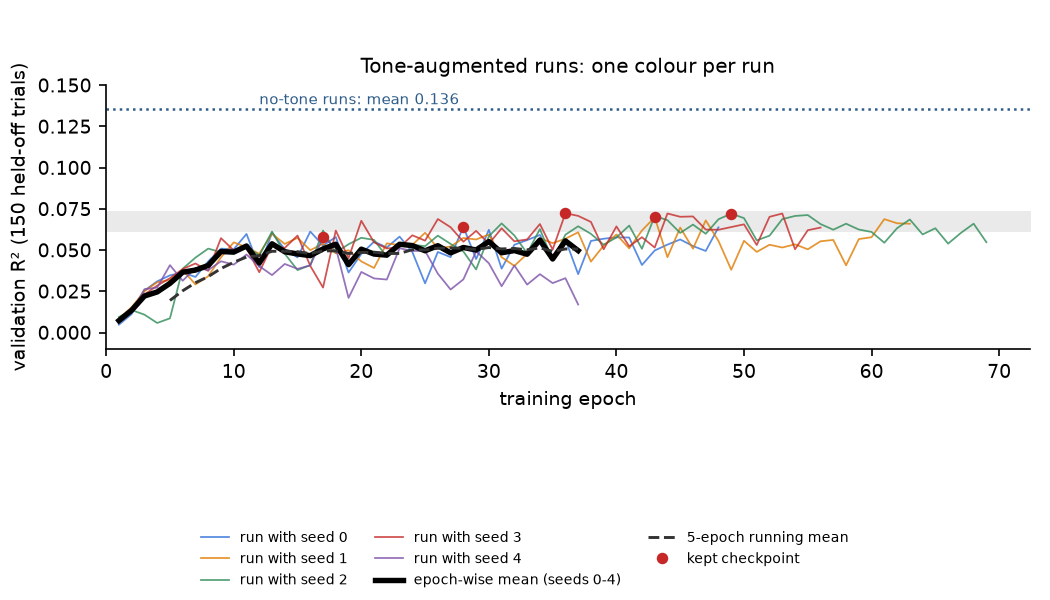
\includegraphics[width=\textwidth]{fig_tones_curves.png}
\caption{Clean validation $R^2$ across training epochs for the five tone-augmented runs. One colour per run; the bold black line is the seed mean, the dashed line its 5-epoch running average, and the red dots mark the kept checkpoints. The dotted line is the unaugmented baseline mean of 0.136, so the whole cluster sits below it: tones buy stimulated robustness at a cost in clean accuracy.}\label{fig:tonescurves}
\end{figure}

\begin{table}[htbp]\centering
\caption{Validation $R^2$ on clean trials for tone-augmented runs.}
\begin{tabular}{@{}lccc@{}}\toprule
Seed & Best validation $R^2$ & Best epoch & Last epoch \\ \midrule
0 & $+0.064$ & 28 & 48 \\ 
1 & $+0.070$ & 43 & 63 \\ 
2 & $+0.072$ & 49 & 69 \\ 
3 & $+0.072$ & 36 & 56 \\ 
4 & $+0.058$ & 17 & 37 \\
\bottomrule\end{tabular}\label{tab:toneseeds}
\end{table}

Tone augmentation lowers clean validation $R^2$ from $0.1357 \pm 0.0112$ to $0.0673 \pm 0.0063$ (Table~\ref{tab:toneseeds}), as models are early-stopped on clean data containing none of the interference they were trained to suppress. On stimulated test sessions (\S\ref{sec:eegnet}), however, the same models improve from $-0.192$ to $+0.032$. While a pure sinusoid only approximates step-and-recover transients, this gain indicates that periodic interference at the modulation frequency drives much of the performance drop.


\section{Why 3~Hz and 20~Hz differ}
\label{app:mechanism}

It is tempting to rank the two modulation frequencies as easier and harder. They are not
ordered that way: for a feature-domain decoder 20~Hz is worse, and for a waveform-domain
decoder 3~Hz is worse by a wide margin. The unifying statement is about period relative to bin
width. At 20~Hz one artifact period equals one 50~ms bin, so binning removes 79\% of the
variance and leaves a lag-1 correlation of 0.98 --- a slow drift that an intercept or a
history window absorbs. At 3~Hz a bin covers a sixth of a cycle, so 56\% survives with a lag-1
correlation of 0.35 --- an oscillation that a linear map cannot fold into an offset.

That statistic, and not raw artifact amplitude, predicts the failures. Across the 14 test
sessions the RMS of the binned term correlates with EEGNet's $\Rtwo$ at Spearman
$\rho=-0.94$, and with the GRU's at $\rho=+0.10$. One 20~Hz session makes the point concretely:
it has the largest raw artifact amplitude in the set (AC RMS 91) yet retains only 1.8\% of it
after binning, and its EEGNet score stays near zero, so judging severity by amplitude alone
would have predicted the wrong answer.

The same reasoning explains why pooling hides the result. Averaging the frequencies together
gives EEGNet an overall score of $-0.145$ that describes neither frequency well ($-0.337$ and
$+0.047$), and makes the ensemble look uniformly bad when it is in fact the best decoder at
20~Hz. Comparisons across decoders should be reported per frequency, with the mechanism in
hand.

\section{Threats to validity}
\label{app:threats}

\emph{Frequency is confounded with day.} All seven 3~Hz sessions fall on three days and all
seven 20~Hz sessions on two. The frequency split reflects a real difference in artifact
structure, but the size of the gap may partly reflect which days were easier to decode.

\emph{Cleaning changes normalisation as well as artifact power.} Each channel is standardised
by its median absolute deviation over the task interval, so a larger artifact inflates the
scale and compresses the neural signal. The MAD ratio is 1.92 at 3~Hz and 1.29 at 20~Hz, so
the cleaned-versus-recorded comparison is not a pure manipulation of artifact amplitude.

\emph{PARRM removes brain activity too.} The filter cannot separate artifact at a given phase
from neural activity at that phase. The cleaned arm is therefore the signal with less artifact
\emph{and} some entrained activity removed, not the signal plus less noise.

\emph{The $10\times$ condition is artificial.} It tests sensitivity to artifact amplitude; it
is not a stronger-stimulation experiment, and it assumes the artifact scales linearly with its
own template.

\emph{This dataset cannot resolve small effects.} With a within-session ceiling near 0.067 and
14 sessions, differences below roughly 0.01 are not measurable. We do not claim that cleaning
contributes exactly nothing after refitting; we claim that no effect is detectable, at a
resolution of about 0.001 to 0.005. The negative result is a bound, not a zero.

\emph{Some archived weights do not reproduce their published rows.} Reloading the ten EEGNet
checkpoints and the two ridge coefficient files reproduces every cached score exactly. The
archived GRU and MLP weights do not: the GRU rescores to 0.031 against a logged 0.031 but with
per-session gaps up to 0.032, and the MLP rescores to $+0.026$ against $-0.012$ with a worst
gap of 0.44. Only one seed of each was kept, so the other seeds cannot be audited. The GRU and
MLP rows are the cached run; the MLP row should not be cited without retraining.

\section{Reproduction}
\label{app:repro}

Every table is regenerated from the saved artifacts, with no training and no tuning:
\begin{verbatim}
  python task4/compare_decoders.py     # tables, intervals, weight audit
  python task4/characterise_amp10_noise.py
  python task4/eval_amp10.py           # the four input arms
\end{verbatim}
The $10\times$ recordings are rebuilt with
\begin{verbatim}
  python semisynthetic/EECS182_make_semisynthetic_h5.py \
      --root data --split val-test --h5-only
\end{verbatim}
and the cleaned-$10\times$ files with \texttt{task4/make\_parrm\_amp10.py}, which also verifies
the re-estimation identity when given \texttt{-{}-verify}. The data layout assumed throughout
is continuous LFP exports, trial tables, kinematics in 50~ms bins, PARRM outputs (cleaned LFP
and artifact estimate) and cached spectral features, under a single data root.

\begin{thebibliography}{9}
\bibitem{lawhern2018}
V.~J. Lawhern, A.~J. Solon, N.~R. Waytowich, S.~M. Gordon, C.~P. Hung, and B.~J. Lance.
EEGNet: a compact convolutional neural network for EEG-based brain--computer interfaces.
\emph{Journal of Neural Engineering}, 15(5):056013, 2018.

\bibitem{schirrmeister2017}
R.~T. Schirrmeister, J.~T. Springenberg, L.~D.~J. Fiederer, M.~Glasstetter, K.~Eggensperger,
M.~Tangermann, F.~Hutter, W.~Burgard, and T.~Ball.
Deep learning with convolutional neural networks for EEG decoding and visualization.
\emph{Human Brain Mapping}, 38(11):5391--5420, 2017.

\bibitem{dastinvanrijn2021}
E. Dastin-van Rijn et al.
PARRM: a method for removing stimulation artifacts from neural recordings.
\emph{Cell Reports Methods}, 1(5):100061, 2021.
\end{thebibliography}

\end{document}
